\section{Projeto da arquitetura}
A arquitetura proposta neste trabalho utiliza os estilos arquiteturais \textit{Client-Server} e \textit{Event-Based}. \textit{Client-Server} pelo fato de um aplicativo consumir algum serviço \textit{RESTFul} sendo neste caso um cliente, enquanto que o serviço \textit{RESTFul} torna-se o servidor. Já o \textit{Event-Based} é um modelo de comunicação baseado em eventos, disposto neste trabalho como um recurso que reduz o nível de acoplamento entre objetos e permite ainda, a comunicação entre partes distintas da aplicação, como por exemplos, os plugins. A arquitetura dispõe de objetos de baixo nível escritos em C++ que trabalham na camada de aplicação, recebendo dados de objetos da camada \textit{UI} e interagem com objetos da camada de \textit{middleware} que realizam a comunicação com o serviço \textit{RESTFul} configurado para o aplicativo, caracterizando a arquitetura como um modelo em camadas. No modelo em camadas, a conexão entre os componentes pode ser realizado tanto por eventos como por objetos compartilhados ou, através de leitura e escrita em um arquivo ou em uma base de dados. Porém, nesta arquitetura, foi utilizado somente eventos para comunicação entre os objetos. A escolha de eventos como principal conector entre os objetos foi feita principalmente por proporcionar comunicação assíncrona entre emissor e ouvinte e pelo fato de não acoplar os componentes, garantindo maior independência entre eles. Outro motivo da escolha de eventos, é o fato do Qt provê nativamente um mecanismo de comunicação através de eventos.\par


\subsection{Tecnologias utilizadas}
As tecnologias utilizadas consiste de todos os elementos necessários para o desenvolvimento deste trabalho. O Qt e o \textit{QtCreator} foram os elementos mais importantes, pois, forneceram os recursos e ferramentas para a construção das principais características da arquitetura. Dentre os recursos providos pelo Qt destaca-se os eventos, que permitem interligar objetos através de sinais e slots\footnote{funções javascript ou métodos de uma classe c++ invocados quando o sinal o qual estão conectados for emitido, recebendo em seus parâmetros os argumentos enviado pelo sinal.} ou \textit{signal handles}, e as APIs providas em classes C++ que integram os recursos da arquitetura, tais como, persistência de dados (via \textit{QSettings} e \textit{QSqlDatabase}) e rede (via \textit{QNetworkAccessManager}). O \textit{QtCreator} é uma IDE que possui recursos integrados à um projeto Qt com destaque para facilidade de \textit{build} do projeto, construção do executável do aplicativo e o \textit{deploy} em um \textit{smartphone}. O \textit{QtCreator} também foi utilizado como editor de código fonte.


\subsection{Etapas de desenvolvimento}
Esta arquitetura foi desenvolvida sob uma metodologia ágil com destaque para uma programação extrema e teste contínuo. A arquitetura recebeu alterações durante 10 meses e a primeira etapa de desenvolvimento introduziu o suporte aos plugins. O primeiro desafio foi desacoplar os plugins do arquivo \textit{qrc}\footnote{qrc – \textit{Qt resource collection} é um arquivo xml que mapeia os arquivos que serão empacotados no aplicativo.} e permitir que a aplicação carregasse-os dinamicamente. Também nesta primeira etapa, foi implementado alguns recursos associados aos plugins, como controle de cache dos arquivos QML, ordenação e \textit{parsing} das páginas (definido pelos plugins), além da criação de um componente genérico a ser extendido por todas as páginas do aplicativo. O controle de cache consiste em regenerar o cache dos arquivos QML após uma atualização para garantir o carregamento de mudanças em cada arquivo a cada release. O componente genérico foi definido como \textit{BasePage.qml}, ele é um objeto da camada \textit{UI} e foi criado para garantir o atendimento de alguns requisitos mínimos de aparência, estrutura e simplificar a criação de páginas.\par

Na segunda etapa, foi implementado classes C++ para gerenciar as configurações da aplicação, uma classe utilitária com métodos a serem invocados pelos plugins para operações de baixo nível que ainda não é suportado pelo QML, além de classes para recursos extra providos pela arquitetura, como por exemplo, uma classe que exibe uma janela de diálogo para seleção de arquivos no dispositivo.\par

Na terceira etapa, foi definido os layouts visuais suportados pela arquitetura e dois modelos foram implementados: O layout em pilha, que faz uso do \textit{container} \textit{StackView} e o layout em linha, que faz uso do \textit{container} \textit{SwipeView}, ambos do \textit{QuickControls}\footnote{módulo do Qt que provê um conjunto de componentes QML para construção de interfaces gráficas.}. Em etapas seguintes, foi desenvolvido componentes visuais reutilizáveis, além das APIs para acesso a rede, notificações do aplicativo e persistência de dados. Os \textit{containers} de layout trabalham na camada \textit{UI} e gerenciam a criação e remoção das páginas do aplicativo. É importante destacar que em ambos os layouts, somente uma página pode ser visualizada por vez. As imagens a seguir apresentam os layouts em pilha e em linha.

\begin{figure}[H]
	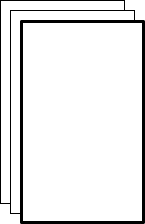
\includegraphics[scale=0.5]{stackview_wireframe}
	\centering
	\caption{Estrutura de um layout em pilha}
\end{figure}

No layout em pilha, o componente \textit{ToolBar.qml} será instanciado e posicionado no topo da janela do aplicativo e trabalhará em conjunto com o \textit{StackView}. O \textit{ToolBar} fará \textit{bindings} com algumas propriedades da página ativa, como por exemplo, adicionando ou removendo botões com ações para a página atual.

\begin{figure}[H]
	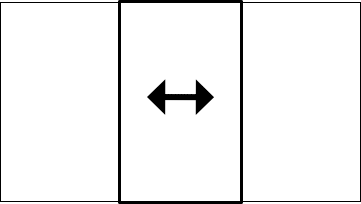
\includegraphics[scale=0.5]{swipeview_wireframe}
	\centering
	\caption{Estrutura de um layout em linha}
\end{figure}

No layout em linha, o componente \textit{TabBar.qml} será instanciado e posicionado no rodapé da janela do aplicativo. O TabBar corresponde ao menu no layout em linha e trabalhará em conjunto com o \textit{SwipeView}. A arquitetura suporta intercalar os dois layouts ao mesmo tempo e um objeto \textit{Binding} do QML manterá o \textit{SwipeView} visível somente quando não houver páginas na pilha do \textit{StackView}. No entanto, o \textit{SwipeView} será instanciado somente se a propriedade \textit{usesSwipeView} for definida para \textit{true} no arquivo de configuração e se tornará o \textit{container} principal. Os objetos correspondentes aos layouts serão instanciados na inicialização e os plugins poderão adicionar ou remover páginas dinamicamente utilizando os identificadores \textit{swipeView} e \textit{pageStack} quando for necessário navegar para uma determinada página a partir de outra, sem ser pelo menu.\par


\subsection{Requisitos funcionais suportados}
O projeto desta arquitetura visa atender quatro requisitos funcionais ententidos como básicos em todo sistema de informação, seja ele mobile ou não. Para atender aos requisitos, foi implementado APIs usando classes C++ nativas do Qt. Apesar de o QML dispôr de funcionalidades que poderiam atender a estes requisitos, foi decidido implementar em C++ por questões de desempenho devido menos código interpretado, melhor controle de consumo de memória e para simplificar a implementação de código nos plugins. Os requisitos listados a seguir, foram disponibilizados na arquitetura através de APIs de alto nível a serem utilizadas pelos plugins. As APIs serão apresentadas em tópicos específicos posteriormente e os requisitos são:

\begin{enumerate}
	\item Acesso a rede para comunicação com serviços \textit{RESTFul};
	\item Persistência de dados local via \textit{SQLITE};
	\item Notificações do aplicativo via \textit{push} e local;
	\item Comunicação entre objetos facilitado.
\end{enumerate}


\subsection{Visão geral da arquitetura}
A figura a seguir, apresenta um diagrama de pacotes e arquivos destacando uma visão lógica dos principais elementos da arquitetura. Em seguida, será descrito a responsabilidade e o conteúdo de cada um deles.

\begin{figure}[H]
	\includegraphics[width=8cm]{diagrama_geral_da_arquitetura}
	\centering
	\caption{Pacotes principais da arquitetura}
\end{figure}

\begin{description}
	\item[1] \textit{main.cpp}: Arquivo inicial da aplicação. Esse arquivo é responsável por instanciar as classes do Qt que exibem a janela do aplicativo e o interpretador de código QML, além de classes da camada de aplicação, configuração e utilitários. O \textit{main.cpp} também é responsável por carregar o arquivo de tradução de acordo com o idioma do dispositivo e registrar objetos no contexto da aplicação a serem utilizados pelos plugins.

	\item[2] \textit{tcc.pro}: Arquivo de configuração de todo projeto Qt. Nele é definido os módulos do Qt a serem utilizados na aplicação, as classes C++ que serão compiladas e linkadas no executável, os aquivos \textit{qrc} que mapeiam os componentes QML, as imagens e arquivos genéricos a serem empacotados no aplicativo, além de módulos e arquivos de configuração para cada plataforma (linux, osx, android e ios). É neste arquivo que fica definido onde os plugins serão instalados no dispositivo.

	\item[3] \textit{config.json}: Arquivo de configuração do aplicativo, pois contém propriedades que indicarão alguns comportamentos iniciais e escolha de tipos de objetos a serem instanciados, tais como, o tipo de layout a ser utilizado, se os termos de uso deve ser exibido na primeira inicialização (carregará o arquivo \textit{assets/eula.html} definido pelo desenvolvedor), se tem login ou não (caso sim, instanciará um objeto que gerencia o perfil do usuário e exibirá a página de login na inicialização) entre outras propriedades. Os detalhes deste arquivo serão apresentados em um tópico mais adiante.

	\item[4] \textit{src}: Diretório de código fonte. É onde está as classes C++, componentes QML utilizados internamente e dispostos para os plugins como reusáveis. Esse diretório está sub-dividido em outros seis diretórios que organizam as classes por tipo de API e são eles:

	\begin{itemize}
		\item \textit{core}: contém classes do núcleo da aplicação dentre elas \textit{App}, \textit{PluginManager}, \textit{Observer}, \textit{Subject} e \textit{Utils}; 

		\item \textit{database}: contém classes da API de persistência de dados;

		\item \textit{extras}: contém classes de customização de estilo no android;

		\item \textit{notification}: contém as classes que gerenciam as notificações baseadas na plataforma;

		\item \textit{network}: contém as classes da API de rede (HTTP);

		\item \textit{qml}: contém os arquivos QML sub-divididos em \textit{private} e \textit{public}, sendo os componentes em \textit{private} os que são utilizados internamente pela aplicação e os que estão em \textit{public} os reutilizáveis.
	\end{itemize}

	\item[5] \textit{plugins}: Diretório de plugins. Cada plugin deve obrigatóriamente estar em um sub-diretório com no mínimo um arquivo de configuração de nome \textit{config.json} e os arquivos QML necessários para o seu funcionamento. Os detalhes dos requisitos para o carregamento de um plugin serão descrito em um tópico posterior.

	\item[6] \textit{translations}: Diretório contendo os arquivos de tradução. Os arquivos de tradução devem ser gerados ou atualizados antes de cada release do aplicativo. Um arquivo de resources \textit{translations.qrc} existe neste diretório e deve ser utilizado para mapear os arquivos de idioma suportados pelo aplicativo. Cada arquivo de tradução deve ser nomeado seguindo o padrão \textit{language\_COUNTRY} com extensão \textit{ts}, por exemplo: \textit{pt\_BR.ts}. Ao iniciar a aplicação, o \textit{main}, tentará identificar o idioma do dispositivo e o arquivo de tradução correspondente (se houver) será carregado para que os textos visíveis sejam traduzidos para o usuário. Para gerar as traduções, deve-se utilizar o comando \textit{lupdate *.pro} (na raíz do projeto) para criar ou atualizar o arquivo \textit{ts} principal.

	\item[7] \textit{android}: Diretório contendo os arquivos de configuração do aplicativo para a plataforma android. Outros sub-diretórios guardam arquivos do \textit{gradle} utilizados para o \textit{build} do APK, ícones do lançador do aplicativo e classes java, além de uma versão da lib \textit{openssl} compilada para o funcionamento de requisições HTTP.

	\item[8] \textit{assets}: Diretório contendo imagens e arquivos de configuração do \textit{qtquickcontrols2}, além de um arquivo html que pode ser usado para exibir os termos de uso do aplicativo quando necessário (se a propriedade \textit{showEula} for definida para \textit{true} no arquivo de configuração). Um arquivo de \textit{resources} \textit{assets.qrc} mapeia todos os arquivos contidos neste diretório.

	\item[9] \textit{ios}: Diretório contendo os arquivos de configuração do aplicativo para a plataforma iOS. Pode conter os ícones do aplicativo e imagens requeridas pela plataforma, tais como as imagens de \textit{splash-screen}, além do arquivo de configuração \textit{Info.plist} que define nome e versão do aplicativo e os recursos do sistema requerido para o funcionamento da aplicação no iOS.
\end{description}


\subsection{Arquitetura de plugins}
As funcionalidades de um aplicativo baseado nesta arquitetura devem ser implementadas através de plugins, atendendo aos requisitos levantados para o aplicativo a ser desenvolvido utilizando apenas QML. Os plugins são independentes entre sí e podem incluir arquivos QML, TXT, HTML e imagens em seu diretório. Qualquer componente de um plugin pode reutilizar os componentes públicos usando a diretiva \textit{import "qrc:/publicComponentes/"}, ao todo quinze componentes foram disponibilizados.\par
Os plugins estão desacoplados do núcleo da aplicação e serão conhecidos em tempo de execução. Ao adicionar um novo plugin no diretório \textit{plugins}, ele será carregado no próximo \textit{build}. Para que um plugin seja identificado pelo objeto gerenciador de plugins e carregado na aplicação, é necessário obedecer as seguintes restrições:

\begin{enumerate}
	\item[1ª] estar em um sub-diretório dentro de \textit{plugins};
	\item[2ª] conter um arquivo \textit{config.json} dentro deste sub-diretório;
	\item[3ª] conter pelo menos um arquivo QML visual ou \textit{listener}.
\end{enumerate}

Os \textit{listeners} são componentes não visuais que observam eventos da aplicação. O arquivo \textit{config.json} de um plugin deve ser um objeto contendo as seguintes propriedades:

\begin{enumerate}
	\item \textit{name} (string): o nome do plugin. Deve ser preenchido para que o plugin seja identificado pelo gerenciador de plugins;

	\item \textit{description} (string): um texto que descreve o plugin. Deve ser definido, caso contrário o plugin não será carregado;

	\item \textit{listeners} (array): uma lista de strings que indentifica os arquivos do plugin (componentes QML não visuais) que serão instanciados como observadores de eventos. O preenchimento dessa propriedade é opcional e pode ser preenchida mesmo que a propriedade \textit{pages} seja preenchida;

	\item \textit{pages} (array): uma lista de objetos que indentifica as páginas do plugin que serão acessadas a partir dos menus do aplicativo e deve ser preenchido se a propriedade \textit{listeners} estiver vazia.
\end{enumerate}

Cada objeto em \textit{pages} poderá conter as seguintes propriedades:

\begin{itemize}
	\item \textit{qml} (string): O nome do arquivo correspondente a página. Se essa propriedade não for definida, a página não será carregada;

	\item \textit{title} (string): O título correspondente a página a ser exibido no menu. Esse valor também é requerido, se não for definido, a página não será adicionada ao menu;

	\item \textit{awesomeIcon} (string) (opcional): O nome de um ícone do \textit{Awesome Icons} que será exibido no menu, em conjunto com o título. Se esse valor não for definido, um ícone padrão (\textit{gear}) será utilizado;

	\item \textit{roles} (array): Uma lista de strings contendo os nomes de perfil de usuário que poderão acessar a página. Essa lista será útil somente se for definido o tipo de perfil do usuário no objeto \textit{userProfile}. O objeto \textit{userProfile} é \textit{null} por default e será instanciado na inicialização do aplicativo se a propriedade \textit{usesLogin} for definida para \textit{true} no arquivo de configuração. Caso \textit{roles} não for definido, será setado um array vazio. Porém, se \textit{userProfile} for instanciado e definido uma string com o perfil do usuário na propriedade \textit{profile} e essa string não tiver em \textit{roles}, a página não será exibida. Informações sobre o objeto \textit{userProfile} será detalhado em um tópico posterior;

	\item \textit{order} (int): Um valor numérico que define a ordem em que a página será exibida na lista de itens nos menus. O desenvolvedor deverá definir um valor acima de zero e quanto maior o valor, maior a prioridade na lista de itens;

	\item \textit{isLoginPage} (bool): Um valor boleano que indica se a página representa a tela de login do aplicativo e deve ser definido pela página correspondente se a propriedade \textit{usesLogin} for definido para \textit{true} no arquivo de configuração. Se o aplicativo usa login, o \textit{path} da página definida como login será persistido pois, será lido por funções internas do aplicativo na inicialização e quando o usuário fizer \textit{logout}. Se mais de uma página for definida como \textit{loginPage} entre os plugins, será utilizada a última página identificada pelo gerenciador de plugins;

	\item \textit{isHomePage} (bool): Um valor boleano que indica se a página corresponde a primeira página exibida para o usuário e deve ser utilizado pela página correspondente quando o layout em pilha estiver sendo utilizado. O \textit{path} dessa página será persistido durante o carregamento dos plugins e será carregada por funções internas na inicialização quando não houver (ou após) o login. Se mais de uma página for definida como \textit{homePage}, será utilizada a última página identificada pelo gerenciador de plugins;

	\item \textit{showInDrawer} (bool): Um valor boleano que indica se a página poderá ser exibida no menu de layout em pilha (\textit{drawer menu}). Por padrão, o menu de layout em pilha será carregado. Porém, poderá ser instanciado no layout em linha se a propriedade \textit{usesDrawer} for definida para \textit{true} no arquivo de configuração. O layout em linha utiliza uma barra de botões como menu e com isso, é possível permitir acesso a páginas diferentes a partir dos dois menus;

	\item \textit{showInTabBar} (bool): Um valor boleano que indica se a página poderá ser exibida no menu de layout em linha. O objetivo dessa propriedade é permitir exibir páginas diferentes nos menus quando o \textit{drawer menu} menu estiver sendo utilizado.
\end{itemize}

As páginas serão instanciadas sob demanda quando o aplicativo tiver utilizando o layout em pilha, neste caso, quando o usuário clicar em um item da lista no menu a página correspondente será instanciada e ficará visível para o usuário. No layout em pilha, o menu é exibido pelo componente \textit{Menu.qml} que consiste de uma instância do objeto \textit{Drawer} do \textit{QuickControls} e as páginas serão listadas verticalmente. Quando o layout em linha estiver sendo utilizado, uma lista horizontal de botões será acidionado no rodapé da janela do aplicativo permitindo ao usuário alternar entre as páginas disponíveis. Porém, no layout em linha, todas as páginas serão instanciadas no início da aplicação e terá um botão associado a cada página. No layout em linha, o menu corresponde ao componente \textit{TabBar.qml} também do \textit{QuickControls} com algumas modificações. As figuras a seguir apresentam um exemplo dos menus utilizado nos layouts em pilha e em linha.

\begin{figure}[H]
	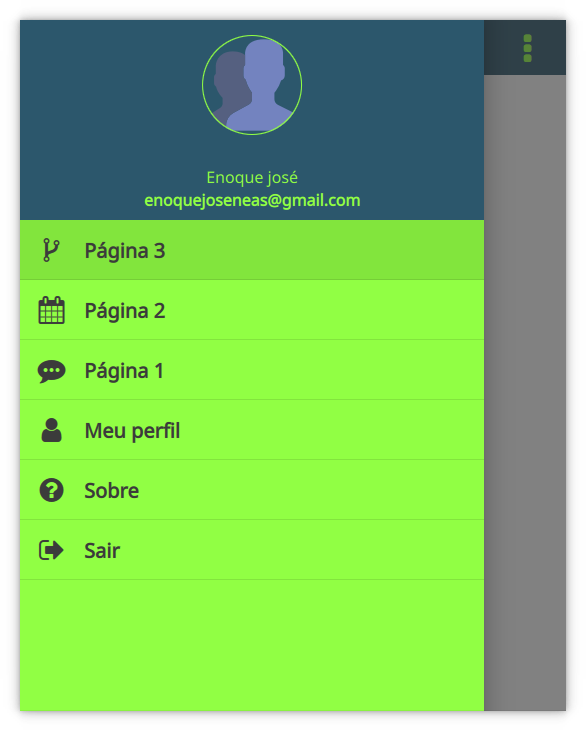
\includegraphics[width=8cm]{exemplo_menu_layout_em_pilha}
	\centering
	\caption{Lista de páginas exibidas no menu de layout em pilha}
\end{figure}

\begin{figure}[H]
	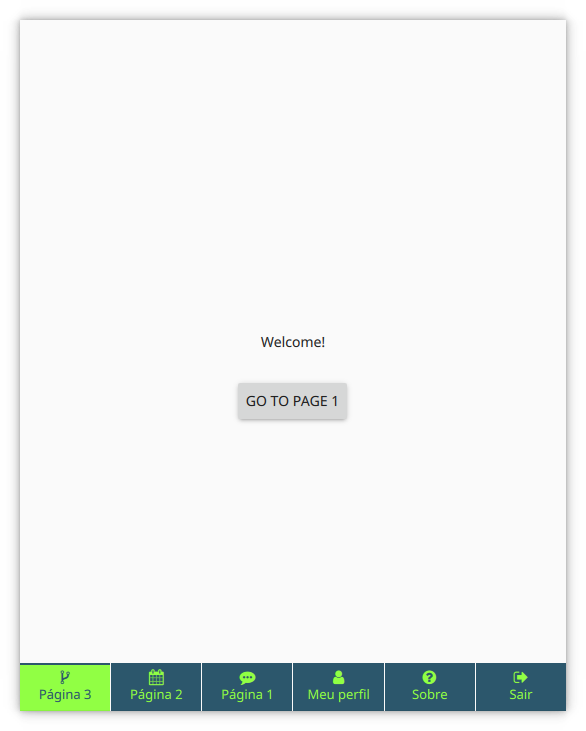
\includegraphics[width=8cm]{exemplo_menu_layout_em_linha}
	\centering
	\caption{Lista de páginas exibidas no menu de layout em linha}
\end{figure}

A exibição do título da página no botão pode ser ocultada setando a opção \textit{showTabButtonText} para \textit{false} no arquivo de configuração.


\subsection{Gerenciamento de plugins}\label{sec:solucao-desenvolvida}
A classe \textit{PluginManager} é responsável por gerenciar os plugins, basicamente, iterando os arquivos dentro do diretório \textit{plugins} e analizando as propriedades do arquivo de configuração de cada plugin. Em cada arquivo, será verificado as propriedades para cada página, adicionando-a como objeto em um array. Após ler todos os plugins, o array de objetos será persistido nas configurações da aplicação para que na próxima inicialização não precise iterar novamente o diretório, lendo as definições dos plugins das configurações. Os plugins serão recarregados após uma atualização do aplicativo ou quando a aplicação for executada em modo \textit{debug}.\par
A cada inicialização, será feito uma verificação da versão do aplicativo, que será persistida nas configurações na primeira execução do aplicativo e atualizada a cada \textit{release}. Se houver diferença entre versão em execução da versão salva na execução anterior, os plugins serão recarregados. Além disso, esta classe também é responsável por deletar todos os arquivos de cache contido no diretório de cache da aplicação a cada \textit{release}. Outra responsabilidade dessa classe, é a criação da tabela do plugin no banco de dados do aplicativo, se existir um arquivo \textit{plugin\_table.sql} no diretório do plugin. O banco de dados da aplicação é criado e gerenciado por outro objeto que controla as operações de persistência e será detalhado em outra seção. O diagrama a seguir, apresenta as operações e atributos da classe \textit{PluginManager}.

\begin{figure}[H]
	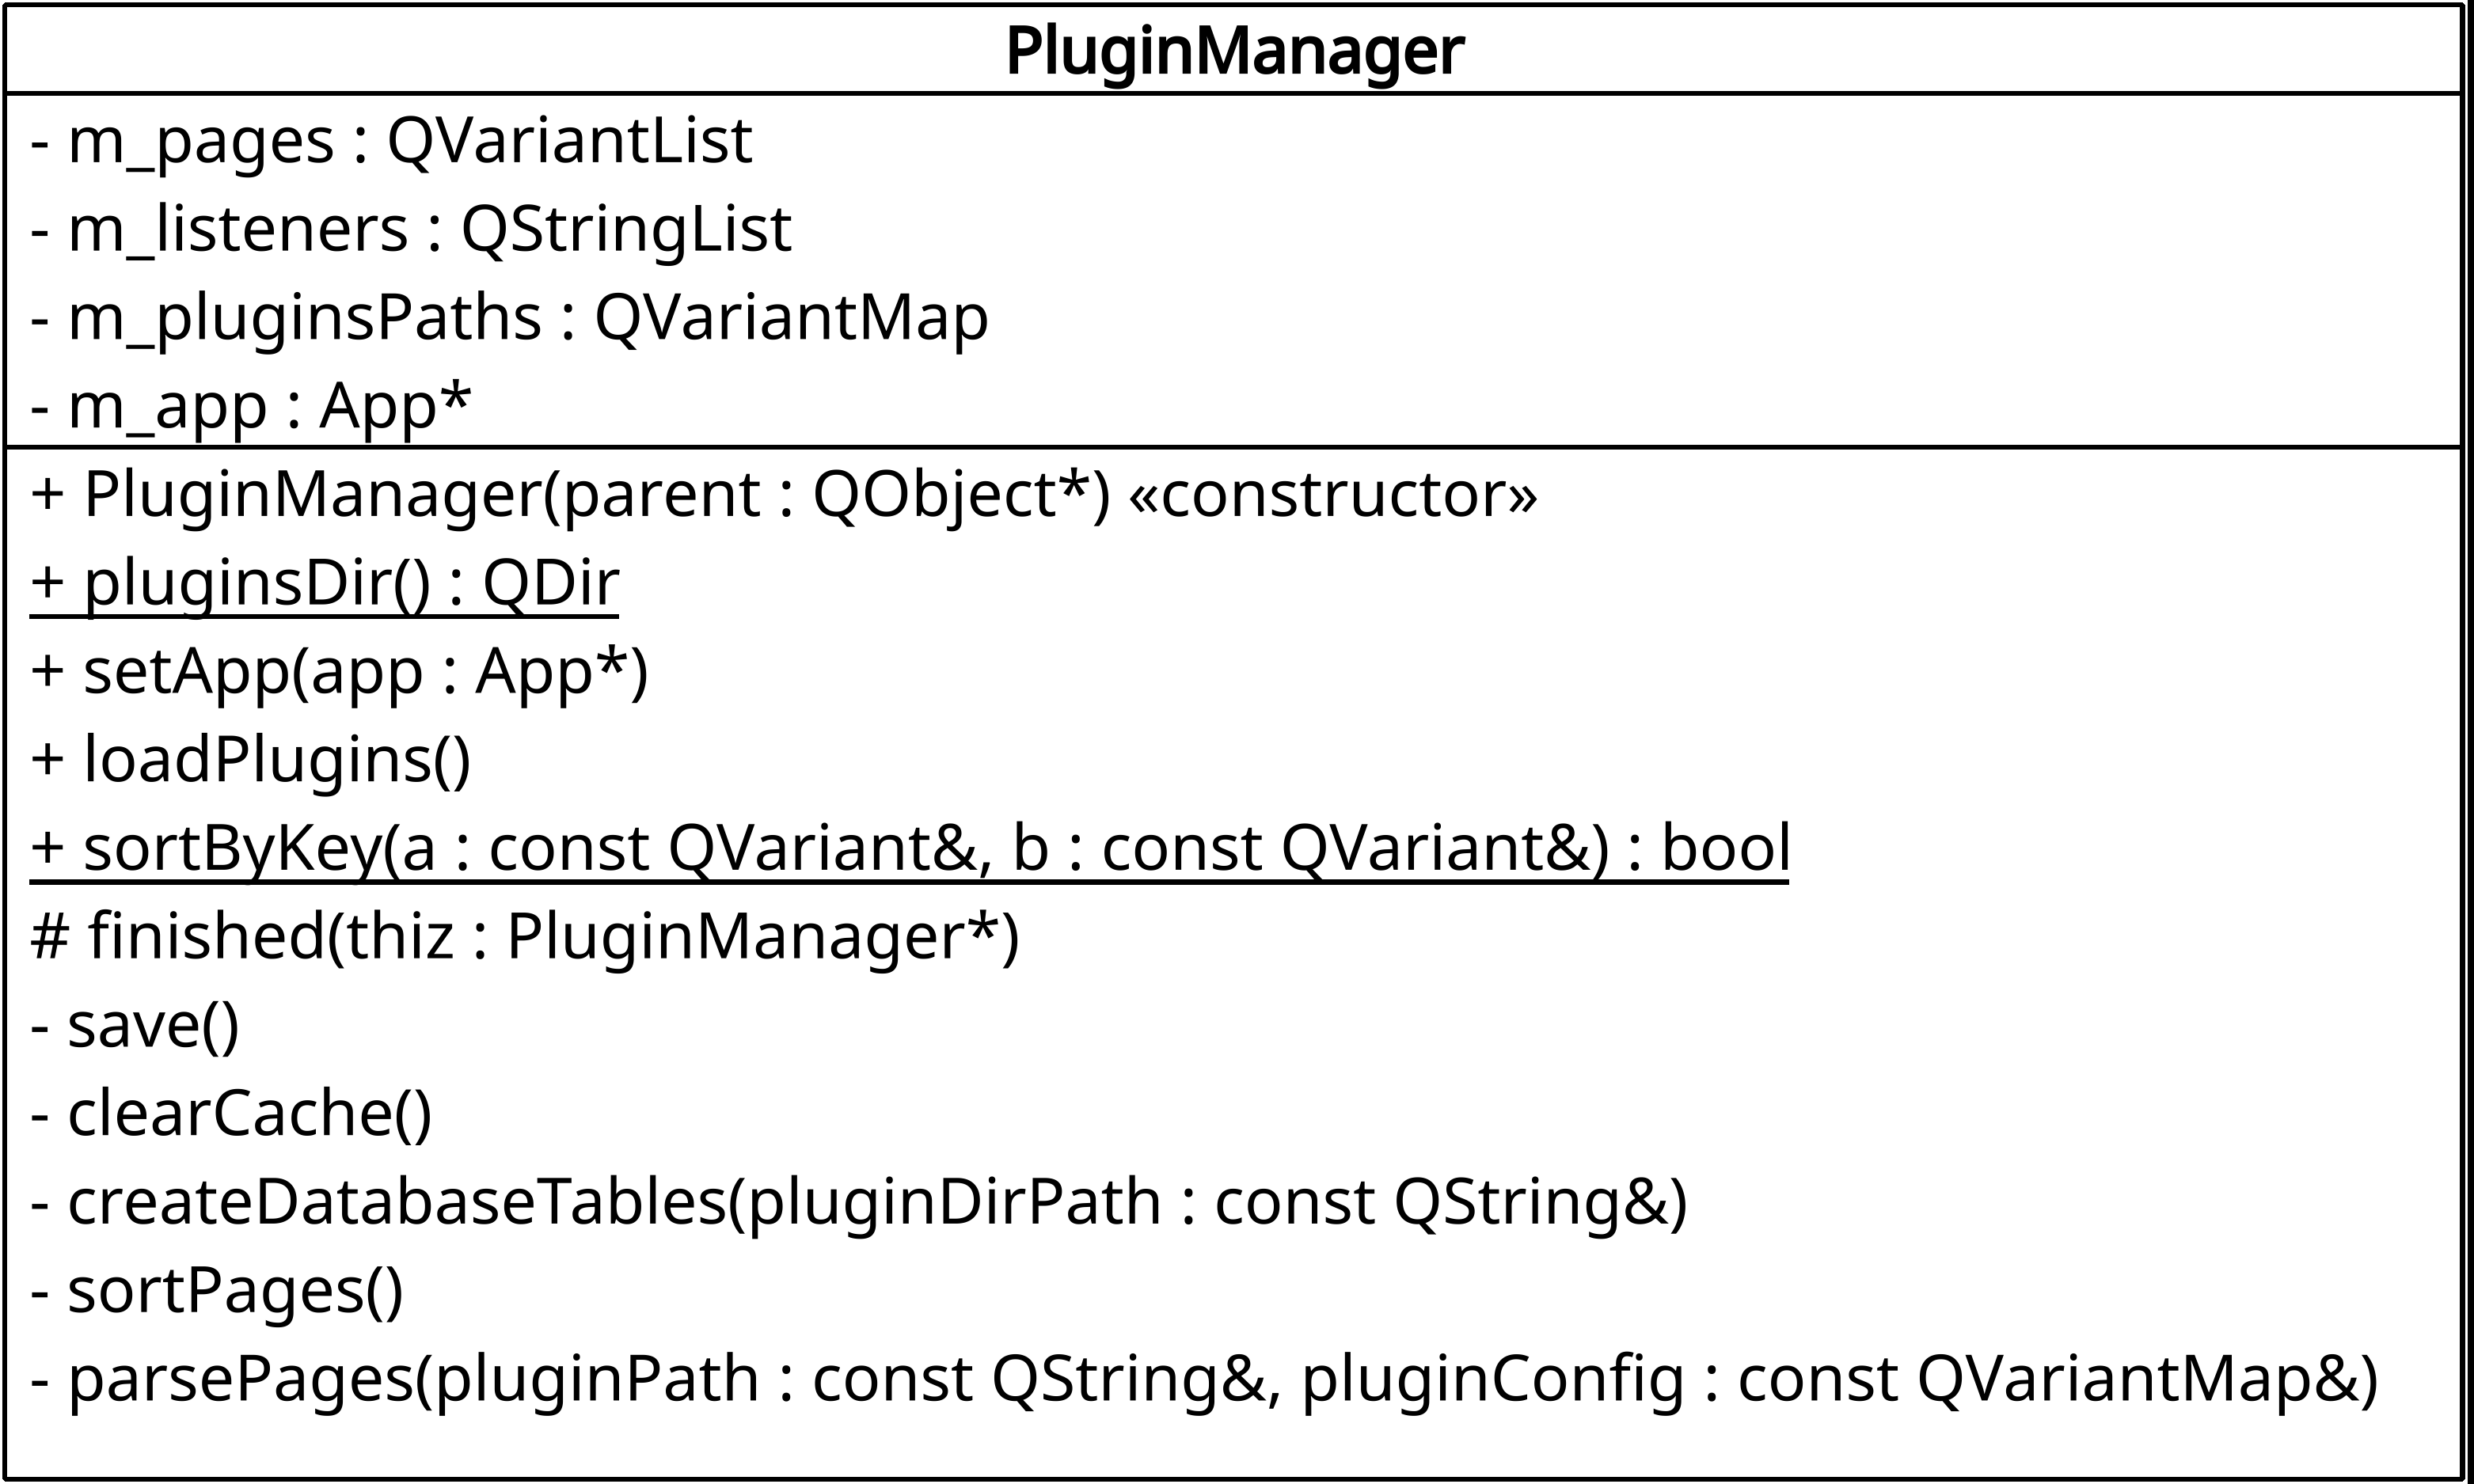
\includegraphics[width=8cm]{diagrama_de_classe_PluginManager}
	\centering
	\caption{Diagrama da classe PluginManager}
\end{figure}

O carregamento dos plugins será feito antes de instanciar qualquer componente visual, na invocação do método \textit{loadPlugins} feito pelo objeto \textit{App}. A instância de \textit{PluginManager} será destruída após o carregamento dos plugins para garantir baixo consumo de memória pelo aplicativo.


\subsection{A classe App}\label{sec:solucao-desenvolvida}
A classe \textit{App} é um componente importante nesta arquitetura, suas principais responsabilidades consiste de instanciar \textit{PluginManager}, carregar o arquivo \textit{config.json} que contém parâmetros da aplicação e gerenciar a persistência das configurações do aplicativo via \textit{QSettings}\footnote{https://doc.qt.io/qt-5/qsettings.html.}. \textit{App} também é responsável por notificar os objetos através do sinal \textit{eventNotify}. A classe \textit{App} será instanciada na inicialização do aplicativo e registrada no contexto da aplicação identificada pela string "App" para que os plugins possam invocar seus métodos públicos. Dentre os métodos possíveis, está o \textit{readSettings} que retorna um tipo genérico de dado requerendo apenas um parâmetro que identifique o valor a ser retornado. Outra tarefa que corresponde a esta classe, é a criação de uma conexão com a atividade do aplicativo no android e no iOS. A aplicação poderá receber parâmetros de eventos como \textit{push notification} ou token de registro no \textit{Firebase}, quando o serviço de \textit{push} for utilizado. O registro do aplicativo no \textit{Firebase} e o recebimento de notificações via \textit{push} é realizado por objetos nativos de cada plataforma em um processo separado da aplicação. Em tempo de execução, as atividade passarão o token e os argumentos recebidos do \textit{push} (título, mensagem, data, etc.) para o aplicativo através de uma chamada ao método estático \textit{fireEventNotify} da classe \textit{App} que irá notificará a aplicação através do sinal \textit{eventNotify}. A figura abaixo apresenta o diagrama da classe \textit{App}.

\begin{figure}[H]
	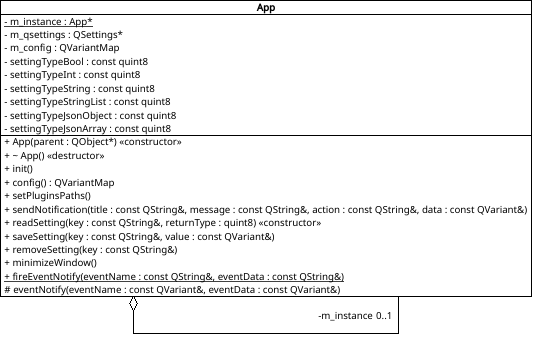
\includegraphics[width=8cm]{diagrama_de_classe_App}
	\centering
	\caption{Diagrama da classe App}
\end{figure}

\textit{App} é quem define o estilo de \textit{widgets} utilizado pelos componentes QML (Material, Universal, etc.). A escolha do estilo deve ser feito pelo desenvolvedor no arquivo de configuração na propriedade \textit{applicationStyle} e será passado diretamente para o objeto \textit{QQuickStyle} na inicialização. Os possíveis valores para esta propriedade serão detalhados na seção que descreve o arquivo \textit{config.json}. A instância da classe \textit{App} adicionará no objeto \textit{Config} uma propriedade contendo o \textit{path} de cada plugin para facilitar o acesso aos arquivos no diretório de cada plugin. Por exemplo, considerando que \textit{Session} é um plugin, os arquivos em seu diretório poderão ser acessados da seguinte forma: \textit{Config.plugins.session + "File.qml"}. O objetivo dessa propriedade é fornecer aos plugins uma forma simplificada de acessar os arquivos em seu diretório, visto que os plugins serão colocados em diretórios virtuais nas plataformas \textit{mobile}: \textit{"assets://"} no android e "Documents/assets\_catalogs://" no ios.


\subsection{Gerenciamento de configurações}
A arquitetura provê uma API simples e de alto nível para persistir dados utilizando o conceito \textit{chave-valor} através do objeto \textit{App}. Nesse modelo de persistência, a chave identifica o dado a ser armazenado e o valor é o dado propriamente dito. Os tipos de dados válidos são: strings, números, objetos ou arrays e os métodos disponíveis podem ler, persistir ou deletar. Os métodos serão descritos a seguir:
	\begin{itemize}
		\item \textit{readSetting}: Utilizado para ler um dado salvo utilizando uma string que identifique a informação a ser retornada. Por padrão, o tipo de retorno é string e se o dado não for string o segundo parâmetro deve ser passado indicando o tipo específico a ser retornado. Os tipos podem ser especificados para evitar o uso de \textit{cast} no QML. Os tipos possíveis são:
		\begin{itemize}
			\item \textit{SettingTypeBool}: para retornar um valor boleano;

			\item \textit{SettingTypeInt}: para retornar um inteiro;

			\item \textit{SettingTypeStringList}: para retornar uma lista de strings;

			\textit{SettingTypeJsonObject}: para retornar um objeto;

			\item \textit{SettingTypeJsonArray}: para retornar um array de objetos.
		\end{itemize}


		\item \textit{saveSetting}: Utilizado para persistir alguma informação. Esse método é \textit{void} e possui dois parâmetros requeridos. O primeiro é uma string que identifica o dado a ser persistido, e o segundo, é o dado propriamente dito. O dado pode ser uma string, um valor numérico, um objeto ou array.

		\item \textit{removeSetting}: Utilizado para apagar alguma informação persistida. Esse método requer apenas um parâmetro, uma string que identifica o dado a ser deletado.
	\end{itemize}

O código a seguir, apresenta um exemplo de persistência e leitura de dados usando o mecanismo \textit{chave-valor}:

\begin{center}
\begin{lstlisting}[language=qml]
import QtQuick 2.8

Item {
    Component.onCompleted: {
		var foo = App.readSetting("foo")
		if (bar != foo)
		   App.saveSetting("foo", bar)
		App.removeSetting("bar")
    }
}
\end{lstlisting}
\captionof{lstlisting}{Exemplo de persistência através do objeto \textit{App}}
\end{center}


\subsection{Gerenciamento de eventos}
A classe \textit{App} possui o sinal \textit{eventNotify} e pode ser utilizado pelos plugins e objetos como conector. Este sinal possui dois parâmetros: o primeiro é uma string que identifica o evento e o segundo, um objeto contendo o dado ou argumento a ser passado para os objetos ouvintes do evento. Como a instância da classe \textit{App} será adicionada ao contexto da aplicação como um objeto global, objetos podem disparar eventos fazendo uma chamada ao sinal da seguinte forma: \textit{App.eventNotify(nome-do-evento, argumento)}. Observadores devem criar uma conexão com este sinal utilizando o objeto \textit{Connections} do QML, especificando como \textit{target} o objeto \textit{App}. O código a seguir, apresenta um exemplo de uma conexão com este sinal:

\begin{center}
\begin{lstlisting}[language=qml]
import QtQuick 2.8
...
Connections {
    target: App
    onEventNotify: {
        if (eventName == Config.events.foo)
            foo()
    }
}
\end{lstlisting}
\captionof{lstlisting}{Exemplo de conexão com o sinal \textit{eventNotify}}
\end{center}


\subsection{O Arquivo de Configuração}\label{sec:solucao-desenvolvida}
O arquivo \textit{config.json} é um componente importante desta arquitetura, ele é utilizado como arquivo de configuração geral do aplicativo, porém, suas informações não são persistidas. O conteúdo deste arquivo será repassado para a aplicação como um objeto javascript e o usuário poderá adicionar propriedades a serem lidas pelos plugins. No entanto, as propriedades fornecidas no modelo desta arquitetura não devem ser removidas, pois, componentes internos fazem uso das propriedades definidas neste arquivo. Os plugins poderão ler essa propriedade acessando \textit{Config.property\_name}. As principais propriedades e seus possíveis valores podem ser entendidas a seguir:

\begin{itemize}
	\item \textit{appName} (string): O nome do aplicativo. Este valor será setado em \textit{QApplication.setApplicationName} na inicialização do aplicativo. Essa informação será útil para Qt identificar as configurações do aplicativo;

	\item \textit{appDescription} (string): Uma descrição sobre o aplicativo. Essa propriedade é opcional;

	\item \textit{organizationName} (string): O nome da organização. Este valor será setado em \textit{QApplication.setOrganizationName} na inicialização do aplicativo e é será utilizado internamente pelo Qt para definir o nome do diretório de configurações da aplicação. Basicamente, será na \textit{home} do usuário (em modo desktop) e no diretório de cache de aplicativos nas plataformas móveis;

	\item \textit{organizationDomain} (string): O endereço do domínio da organização, por exemplo, \textit{qt.project.org}. Será utilizado pelo Qt internamente;

	\item \textit{applicationStyle} (string): O nome do estilo a ser aplicado nos \textit{widgets} (\textit{Button}, \textit{TabBar}, \textit{ToolTip} e etc.). Os possíveis valores são: \textit{Material}, \textit{Universal} ou \textit{Default}. O valor dessa propriedade será passada pelo objeto \textit{App} para \textit{QQuickStyle};

	\item \textit{forceEulaAgreement} (bool): Um valor boleano que inidica se a aplicação deverá exigir do usuário confirmação de aceitação dos termos de uso para continuar usando o aplicativo. Esse valor só terá efeito se a propriedade \textit{showEula} for definida para \textit{true};

	\item \textit{hasLogin} (bool): Um valor boleano que indica se o aplicativo deverá carregar uma página de login na inicialização. Se for definido para \textit{true}, a aplicação irá utilizar a página (dentre os plugins) que definiu \textit{isLoginPage} para \textit{true}, identificada pelo gerenciador de plugins durante o carregamento dos plugins;

	\item \textit{showEula} (bool): Um valor boleano que inidica se a aplicação exibirá para o usuário uma página contendo os termos de uso do aplicativo. Caso seja setado para \textit{true}, o arquivo \textit{assets/eula.html} será carregado e exibido na primeira execução do aplicativo. Após o usuário ler e aceitar os termos de uso, o usuário irá para a página de login ou a \textit{home page} se tiver sido definida;

	\item \textit{showTabButtonText} (bool): Um valor boleano que indica se o título da página será exibida nos botões do menu em linha (\textit{TabButton} do \textit{QuickControls}). Essa propriedade só terá efeito quando a aplicação tiver usando o layout em linha;

	\item \textit{usesSwipeView} (bool): Um valor boleano que indica se o layout principal do aplicativo será em linha, que consiste na utilização de um container do \textit{QuickControls} \textit{SwipeView}. No entanto, o container responsável pelo layout em pilha, \textit{StackView} ainda continuará disponível na aplicação, porém como container secundário. Um objeto fará o \textit{Binding} entre ambos os containers, ocultando o \textit{SwipeView} quando alguma página for adicionada a pilha do \textit{StackView}. No \textit{SwipeView} o usuário poderá alternar entre as páginas deslizando horizontalmente.

	\item \textit{usesDrawer} (bool): Um valor boleano que indica se o menu lateral usado no layout em pilha, será instanciado. Esse componente corresponde ao \textit{Drawer} do \textit{QuickControls}. No entando, esse \textit{flag} terá efeito apenas no layout em linha, ou seja, se \textit{usesSwipeView} for \textit{true}, pois no layout em pilha ele será instanciado mesmo que esse \textit{flag} seja \textit{false}. O objetivo dessa propriedade é permitir que o programador possa utilizar o menu lateral quando o layout for em linha, intercalando as páginas que serão visíveis em cada um dos menus através das propriedades \textit{showInDrawer} e \textit{showInTabBar} na configuração das páginas nos plugins;

	\item \textit{showDrawerImage} (bool): Um valor boleano que indica se a imagem do \textit{Drawer} menu será carregada. Por padrão a imagem não será exibida.

	\item \textit{restService} (object): Um objeto contendo as definições do serviço \textit{REST}, como url base e os parâmetros de autenticação básica, usuário e senha. O valor informado em \textit{userName} e \textit{userPass} serão passados em cada requisição HTTP como token baseado em um \textit{hash} \textit{base64}. As seguintes propriedades são requeridas:

	\begin{itemize}
		\item \textit{userName} (string): O nome do usuário do serviço \textit{REST};

		\item \textit{userPass} (string): A senha de usuário do serviço \textit{REST};

		\item \textit{baseUrl} (string): A url base do serviço REST. Essa propriedade será utilizada pelo objeto \textit{RequestHttp} nos métodos de requisições \textit{GET}, \textit{POST} e etc. A sugestão é que nas páginas que fazem requisições HTTP adicione apenas o \textit{path}, a fim de reduzir e simplificar o código. Com isso, uma alteração futura da url do serviço REST seria feita apenas no arquivo de configuração. Internamente, o objeto que realiza a requisição concatenará essa propriedade com o \textit{path} passado no primeiro parâmetro do método;

		\item \textit{baseImagesUrl} (string): A url base dos arquivos de imagens, caso o serviço \textit{REST} utilize uma url diferente ou um sub-domínio para os \textit{resources}.
	\end{itemize}

	\item \textit{fontSize} (object): Um objeto com as definições de valores inteiros para os tamanhos de fonte a serem utilizadas em elementos textuais tais como o \textit{Label}. Essa propriedade possui 4 atributos: \textit{small}, \textit{normal}, \textit{large} e \textit{extraLarge};

	\item \textit{theme} (object): Um objeto com as definições de cores utilizada nos elementos visuais, tais como Botões, \textit{ToolBar}, \textit{TabBar}, cor de fundo das páginas;

	\item \textit{events}: (object): Um objeto que mapeia os eventos, baseados em um par de strings \textit{nome-do-evento.valor}. Essa propriedade será utilizada por objetos e componentes internos para identificar de qual evento estão sendo notificados, a fim de padronizar os nomes dos eventos e reduzir a replicação de strings na aplicação. Essa propriedade poderá ser utilizado tanto em conexões com o sinal \textit{eventNotify} do objeto App como pela API do \textit{Observer} disponibilizado pela arquitetura (será detalhado em um seção mais adiante). O objeto \textit{App} adicionará treze eventos a essa propriedade na inicialização do aplicativo, alguns deles serão utilizados somente por objetos internos, outros podem ser utilizados pelos plugins para executarem ações específicas em dado momento. Esses eventos serão descritos a seguir:

	\begin{itemize}
		\item \textit{cameraImageSaved} (string): Utilizado para notificar observadores de que uma imagem foi capturada pela câmera do dispositivo e salva localmente. A url da imagem salva será passado no argumento do evento;

		\item \textit{cancelSearch} (string): Utilizado pelo \textit{ToolBar} para indicar que o campo de busca não está ativo, para que a página corrente atualize o conteúdo para o usuário. O \textit{ToolBar} possui um campo texto para pesquisa e ficará visível quando a página alterar o valor da propriedade \textit{toolBarStatus} para \textit{"search"}. Essa funcionalidade permitirá que uma página filtre os resultados exibidos na sua \textit{view}, recebendo em um atributo string \textit{searchText} o valor digitado no campo. O usuário poderá cancelar a busca clicando em um botão voltar que ficará visível ao lado esquerdo do campo de busca e nesse momento, este evento será disparado;

		\item \textit{logoutApplication} (string): utilizado pelo objeto \textit{UserProfile} para atualizar o status da propriedade \textit{isUserLoggedIn} para \textit{false} e em seguida carregar na página de login;

		\item \textit{newActionNotification} (string): utilizado para notificar a aplicação quando o usuário clicar em uma notificação e o aplicativo ficar em \textit{foreground}, vale para notificações via \textit{push} e local. Esse evento será disparado pela atividade do Android (\textit{CustomActivity}) e pelo objeto \textit{QtAppDelegate} no iOS e repassado para a aplicação através do objeto \textit{App}. O argumento do evento (\textit{eventData}) conterá os dados da mensagem em uma string sendo necessário fazer o \textit{parsing} caso seja um objeto json;

		\item \textit{newPushNotification} (string): utilizado sempre que uma notificação via \textit{push} chegar no dispositivo e o mesmo estiver em execução, em \textit{foreground} ou \textit{background}. Ele será disparado a partir dos serviços de notificação que executam em outro processo e serão repassados para a aplicação através de uma conexão entre o objeto java \textit{CustomAtivity} no android e o \textit{QtAppDelegate} no iOS. O argumento do evento (\textit{eventData}), conterá os dados da mensagem em uma string sendo necessário fazer o \textit{parsing} caso seja um objeto json;

		\item \textit{newPushNotificationToken} (string): utilizado quando o registro no \textit{Firebase} for realizado com sucesso. Esse evento será disparado por objetos que executam em outro processo e serão passados para a aplicação através de uma conexão entre o objeto java \textit{CustomAtivity} no android e o \textit{QtAppDelegate} no iOS. O argumento do evento (\textit{eventData}) conterá o token em uma string;

		\item \textit{openDrawer} (string): utilizado intermante para abrir o menu do layout em pilha quando o usuário clicar no botão de menu, posicionado no canto esquerdo do \textit{ToolBar}. O menu do layout em pilha fica oculto por padrão e o usuário poderá torná-lo visível arrastando da esquerda para a direita na janela do aplicativo;

		\item \textit{popCurrentPage} (string): Esse evento deverá ser disparado quando for necessário remover a página ativa da pilha do \textit{StackView}. Será disparado internamente pelo \textit{ToolBar} quando o usuário clicar no botão voltar (seta para a esquerda, exibido se a página definir a propriedade \textit{toolBarState} para \textit{"goBack"}) ou quando o botão \textit{back-button} do android for pressionado. O \textit{StackView} por exemplo, removerá a página da pilha quando este for emitido;

		\item \textit{appendOptionPage} (string): Esse evento pode ser utilizado para adicionar um novo item na lista de opções do menu. Esse evento poderá ser utilizado em ambos os layouts em pilha ou em linha e o argumento do evento deve ser um objeto contendo as propriedades de uma página utilizado no \textit{config.json} de um plugin;

		\item \textit{requestUpdateUserProfile} (string): Esse evento deve ser emitido quando houver um perfil de usuário no aplicativo e permitirá atualizar as informações ou dados do usuário no objeto \textit{UserProfile}. Por exemplo, uma página que permite editar os dados do usuário em um formulário, após o usuário atualizar alguma informação, a página poderá emitir esse evento passando como argumento um objeto contendo as informações do usuário no estilo \textit{chave-valor}.

		\item \textit{initUserProfile} (string): Esse evento deve ser utilizado quando houver um perfil de usuário e um objeto contendo os dados do usuário deverá ser passado no argumento do evento, contendo no mínimo as propriedades \textit{id} e \textit{email}. Um exemplo de uso deste evento, pode ser feito pela página de login, após sucesso na autenticação. A página de login poderá emitir esse evento, passando como argumento o objeto retornado pelo serviço \textit{REST}. O objeto \textit{UserProfile} observa esse evento e quando o mesmo for emitido, ele irá salvar os dados do usuário no objeto \textit{profile} e em seguida, atualizar a propriedade \textit{isLoggedIn} para \textit{true} e carregará a \textit{home page};

		\item \textit{setUserProfileData} (string): Esse evento também deve ser utilizado quando houver um perfil de usuário e permitirá adicionar ou atualizar uma informação no perfil do usuário. Logo, o argumento do evento deve conter a propriedade \textit{key} indicando o nome da propriedade a ser adicionada e \textit{value} contendo o respectivo valor. Por exemplo, o seguinte objeto pode ser utilizado como argumento deste evento: \textit{\{"key": "username", "value": "enoque"\}};

		\item \textit{userProfileChanged} (string): Esse evento será disparado pelo objeto \textit{UserProfile} sempre que ocorrer alguma atualização nos dados do usuário. No argumento do evento será passado uma referência para o objeto \textit{profile}.
	\end{itemize}
\end{itemize}


\subsection{Acesso a Rede (HTTP)}\label{sec:solucao-desenvolvida}
O primeiro requisito funcional provido na arquitetura é o acesso a rede para comunicação com serviços \textit{RESTFul}. Para permitir o uso de rede pelos plugins, foi criado uma classe C++ que realiza requisições HTTP com suporte a autenticação básica, \textit{download} e \textit{upload} de arquivos. O objetivo dessa classe é oferecer um componente rico em recursos, com bom desempenho e fornecer um componente de alto nível para os plugins. Essa classe utiliza componentes do Qt e entregará a resposta de cada requisição em objetos json dispensando o uso de \textit{cast} pelos objetos. Para entregar uma API ainda mais fácil de utilizar, foi criado um componente QML com o mesmo nome da classe e disponibilizado como reusável. Para simplificar o acesso a rede, o desenvolvedor deverá adicionar na propriedade \textit{restService} no arquivo de configuração, a url do serviço \textit{REST} em \textit{baseUrl}, o nome e a senha do usuário da API em \textit{userName} e \textit{userPass} respectivamente e utilizar apenas o \textit{path} da url nos métodos de requisições. As subseções a seguir, descrevem os detalhes da classe \textit{RequestHttp} e do componente correspondente.

\subsubsection{A classe RequestHttp}\label{sec:solucao-desenvolvida}
A classe \textit{RequestHttp} utiliza a classe \textit{QNetworkAccessManager} para gerenciar as operações de rede abstraindo para o aplicativo a interface de rede utilizada no dispositivo. Os métodos disponíveis inicialmente são \textit{GET} e \textit{POST}, além de \textit{download} de arquivos via \textit{GET} e \textit{upload} de arquivos via \textit{POST} ou \textit{PUT}. A classe \textit{QNetworkRequest} do Qt será utilizada para encapsular os parâmetros da requisição. Os métodos principais dessa classe serão descritos a seguir:

\begin{itemize}
	\item \textit{get}: realiza uma requisição do tipo \textit{GET} exigindo apenas a url de destino. Esse método possui dois parâmetros opcionais, o primeiro deles é um objeto do tipo \textit{chave-valor} e se for passado, adicionará a url uma \textit{query-string}. O segundo parâmetro opcional é também um objeto e pode ser passado quando for necessário adicionar dados no cabeçalho da requisição. O código a seguir, apresenta um exemplo de uso desse método:

\begin{center}
\begin{lstlisting}[language=qml]
import QtQuick 2.8
import "qrc:/publicComponents" as Components

Components.RequestHttp {
	id: requestHttp
}
...
Item {
	Component.onCompleted: {
		var queryString = {
			"someKey": "foo",
			"paginate": listView.count
		}
		requestHttp.get("foo", queryString)
	}
}
\end{lstlisting}
% não está ficando centralizada
% \captionof{lstlisting}{Exemplo de uma requisição do tipo \textit{GET}}
\end{center}


	\item \textit{post}: realiza uma requisição do tipo \textit{POST} exigindo a url de destino e o dado a ser postado em formato string. O terceiro parâmetro desse método é opcional e pode ser passando quando for necessário adicionar dados no cabeçalho da requisição. O código a seguir, apresenta um exemplo de uso do método post:

\begin{center}
\begin{lstlisting}[language=qml]
import QtQuick 2.8
import "qrc:/publicComponents" as Components
	
Components.RequestHttp {
	id: requestHttp
}
...
Item {
	Component.onCompleted: {
		var postData = JSON.stringfy({
			"someKey": "bar",
			"email": textField.text
		})
		requestHttp.post("bar", postData)
	}
}
\end{lstlisting}
% não está ficando centralizada
% \captionof{lstlisting}{Exemplo de uma requisição do tipo \textit{POST}}
\end{center}


	\item \textit{uploadFile}: realiza uma requisição do tipo \textit{POST} ou \textit{PUT} exigindo a url de destino e um array de strings contendo os endereços dos arquivos locais a serem enviados para o servidor. A requisição será do tipo \textit{multipart-formdata} e do tipo \textit{POST} (por default). O terceiro parâmetro (boleano, default \textit{false}) pode ser passado quando for necessário utilizar o método \textit{PUT}. Já o último parâmetro, poderá ser passado quando for necessário adicionar dados no cabeçalho da requisição. Esse método emitirá o sinal \textit{uploadFinished} para cada arquivo enviado. Durante o upload de cada arquivo, será emitido o sinal \textit{uploadProgressChanged} contendo os bytes do arquivo (local) e o total de bytes já enviados para o servidor. O código a seguir, apresenta um exemplo de uso desse método:

\begin{center}
\begin{lstlisting}[language=qml]
import QtQuick 2.8
import "qrc:/publicComponents" as Components
	
Components.RequestHttp {
	id: requestHttp
}
...
Item {
	Component.onCompleted: {
		var files = [
			"/data/app/myapp/files/f1.png",
			"/data/app/myapp/files/f2.png"
		]
		requestHttp.upload("bar", files)
	}
}
\end{lstlisting}
% não está ficando centralizada
% \captionof{lstlisting}{Exemplo de uma requisição de \textit{upload} de arquivos}
\end{center}


	\item \textit{downloadFile}: realiza uma requisição do tipo \textit{GET} exigindo apenas uma lista de urls de arquivos a serem baixados para o dispositivo. Por padrão, os arquivos serão salvos no diretório público de \textit{downloads} no dispositivo. No entanto, o segundo parâmetro \textit{saveInAppDirectory} (boleano, default \textit{false}) pode ser utilizado para alterar o diretório de destino dos arquivos para uma pasta interna do aplicativo. Para cada arquivo salvo, o sinal \textit{downloadedFileSaved} será emitido passando o \textit{path} do arquivo salvo localmente. Outro sinal \textit{downloadProgressChanged} será emitido passando dois argumentos, o primeiro indica o total de bytes do arquivo que está sendo baixado e o segundo, um valor inteiro indicando os bytes já baixados. O código a seguir, demonstra um exemplo de requisição para download de arquivos:

\begin{center}
\begin{lstlisting}[language=qml]
import QtQuick 2.8
import "qrc:/publicComponents" as Components
	
Components.RequestHttp {
	id: requestHttp
}
...
Item {
	Component.onCompleted: {
		var urls = [
			"https://.../files/f1.png",
			"https://.../files/f2.png"
		]
		requestHttp.downloadFile(urls)
	}
}
\end{lstlisting}
% não está ficando centralizada
% \captionof{lstlisting}{Exemplo de uma requisição de \textit{upload} de arquivos}
\end{center}

\end{itemize}

Os métodos descritos anteriormente são todos \textit{void}, assíncronos e são declarados como \textit{Q\_INVOKABLE} \footnote{htps://doc.qt.io/qt-5/qtQML-cppintegration-exposecppattributes.html} para permitir o uso dos métodos em componentes QML, como é o caso do componente \textit{RequestHttp}. Para obter a resposta de uma requisição, é preciso criar uma conexão com o sinal \textit{finished}. Esse sinal será emitido por todos os métodos descritos anteriomente se não houver erros no pedido e logo após o envio da resposta pelo servidor. O sinal \textit{finished} passará dois argumentos, \textit{statusCode}, um valor inteiro indicando o status da resposta (200, 400, 500, etc.) e \textit{response} contendo o dado enviado pelo servidor. Se a resposta enviada pelo servidor for um json válido, \textit{response} conterá um objeto ou array, caso contrário, uma string contendo o dado bruto.\par

O sinal \textit{error} será emitido quando houver erros em um pedido e passará dois argumentos, \textit{statusCode} (integer) indicando o código HTTP correspondente ao erro, e \textit{message} (string) contendo a mensagem do erro.\par

A propriedade \textit{status} (integer) declarada como \textit{Q\_PROPERTY} indicará o \textit{status} atual de uma requisição. Essa propriedade pode ser comparada com qualquer uma das seguintes meta-propriedades (útil para fazer \textit{bindings} com outros objetos):

\begin{itemize}
	\item \textit{Error}: inidica um erro no pedido, quando o servidor não responder ou o status da requisição for zero;

	\item \textit{Finished}: indica que a requisição terminou e é setada em \textit{status} antes da emissão do sinal \textit{finished};

	\item \textit{Loading}: indica que a requisição está em andamento ou carregando;

	\item \textit{Ready}: indica que a requisição está pronta, será setada em \textit{status} no construtor do objeto \textit{RequestHttp} e logo após a emissão do sinal \textit{finished}.
\end{itemize}

O diagrama a seguir, apresenta os atributos e métodos da classe \textit{RequestHttp}:

\begin{figure}[h]
	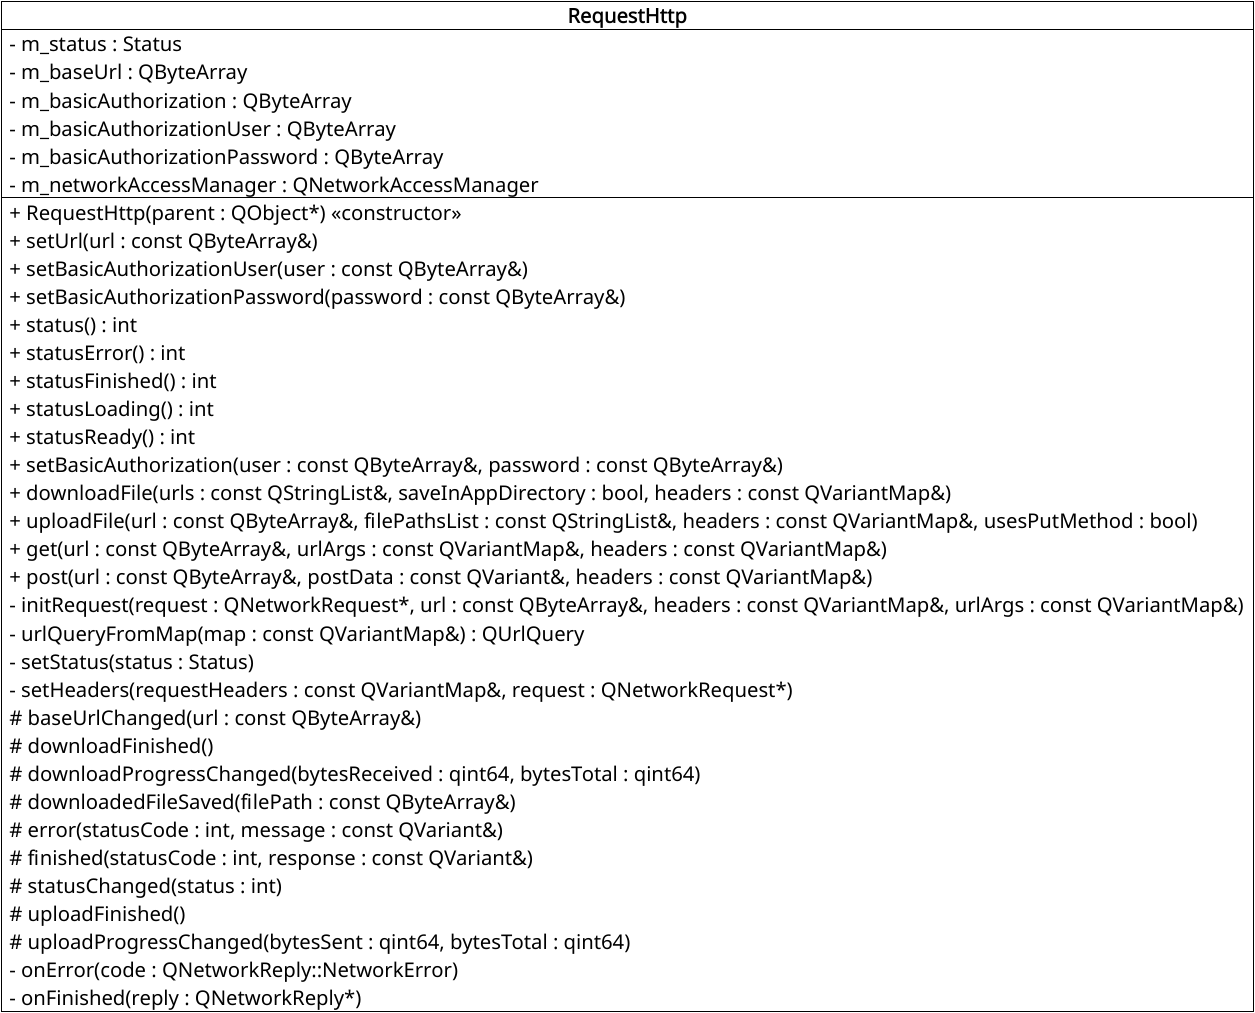
\includegraphics[width=8cm]{diagrama_de_classe_RequestHttp}
	\centering
	\caption{Diagrama da classe \textit{RequestHttp}}
\end{figure}

\subsubsection{O Componente RequestHttp}\label{sec:solucao-desenvolvida}
A classe \textit{RequestHttp} será registrada como um tipo QML no contexto da aplicação e para ser instanciada basta adicionar a diretiva \textit{import RequestHttp 1.0} e em seguida, declarar um objeto QML. No entando, para simplificar ainda mais o uso de rede, os plugins podem utilizar o componente \textit{RequestHttp} que instancia a classe \textit{RequestHttp} e inicializa os atributos \textit{baseUrl} e os parâmetros de autenticação, além de exibir mensagens de erro personalizada para o usuário. Os exemplos de código apresentados na subseção anterior, utilizam o componente \textit{RequestHttp} importando-o dos arquivos reusáveis. No entanto, objetos \textit{listeners} que por algum motivo não utilizem o serviço \textit{REST}, podem instanciar a classe \textit{RequestHttp} diretamente. O código a seguir, apresenta um exemplo de uso da classe \textit{RequestHttp}:

\begin{center}
\begin{lstlisting}[language=qml]
import RequestHttp 1.0 

RequestHttp {
    baseUrl: Config.restService.baseUrl
    authorizationUser: Config.restService.userName
    authorizationPass: Config.restService.userPass
    onError: {
     var message = "Erro ao conectar no servidor"
        if ("android" == Qt.platform.os)
	        snackbar.show(message)
		else
	        functions.alert("Error!", message)
    }
}
\end{lstlisting}
\captionof{lstlisting}{Código do componente \textit{RequestHttp.qml}}
\end{center}


\subsection{Persistência de Dados}\label{sec:solucao-desenvolvida}
Persistência de dados é o segundo requisito funcional disponibilizado nesta arquitetura e visa fornecer aos plugins a possibilidade de persistir dados em um banco \textit{SQLITE} e o funcionamento \textit{offline} do aplicativo. Cada plugin pode criar uma ou mais tabelas no banco de dados e realizar as operações de inserção, atualização e busca de dados em suas tabelas, basta importar o componente \textit{Database} com a diretiva \textit{import Database 1.0} e utilizá-lo como componente QML. Para criar as tabelas no banco de dados do aplicativo, o plugin deve fornecer um arquivo \textit{plugin\_table.sql} contendo os comandos de criação, alteração ou remoção das tabelas. A cada release, esse arquivo será carregado e executado como uma \textit{query} sql permitindo aos plugins atualizar as tabelas (adicionar, remover ou modificar as colunas) quando for necessário.\par

Para gerenciar as operações de banco de dados, foi criado uma classe C++ chamada \textit{Database} que encapsula em métodos de alto nível as operações necessárias para criar o banco de dados, conectar e executar as operações sql. No entanto, essa classe não será utilizada pelos plugins diretamente, foi criado outra classe chamada \textit{DatabaseComponent} que agrega uma instância de \textit{Database} e delega as operações para esse objeto e fornece alguns recursos para simplificar ainda mais a persistência de dados. As subseções a seguir apresentam detalhes de ambas as classes \textit{Database} e \textit{DatabaseComponent}.

\subsubsection{A classe Database}\label{sec:solucao-desenvolvida}
A classe \textit{Database} é responsável por criar o banco de dados \textit{SQLITE} na primeira execução do aplicativo se houver necessidade, ou seja, se algum plugin dispor de um arquivo \textit{plugin\_table.sql} em seu diretório. Se nenhum plugin fornecer esse arquivo, o banco de dados \textit{SQLITE} não será criado. A classe \textit{Database} utiliza as classes \textit{QSqlDatabase} para criação e conexão com o banco de dados e as classes \textit{QSqlQuery} e \textit{QSqlRecord} para as realizar \textit{querys} e retornar os resultados das cosultas. Os métodos principais desta classe serão descritos a seguir:

\begin{itemize}
	\item \textit{select}: esse método pode ser utilizado para recuperar dados de uma tabela através de uma consulta \textit{sql} e possui três parâmetros, o primeiro é nome da tabela onde será feito a consulta, o segundo é um objeto contendo os parâmetros da consulta (condição \textit{where}) no estilo \textit{nome-da-coluna.valor}, e o último parâmetro, um outro objeto contendo argumentos adicionais, tais como \textit{limit}, \textit{offset} e \textit{order by}. Esse método retornará uma lista de objetos resultante da consulta, e cada objeto contido na lista é composto de \textit{nome-da-coluna.valor}. Se a consulta não for efetuada com sucesso, será retornado uma lista vazia;

	\item \textit{insert}: esse método pode ser utilizado para inserir dados em uma tabela e os parâmetros requeridos são: o nome da tabela onde será feito a inserção e um objeto no estilo \textit{nome-da-coluna.valor} contendo os dados a serem persistidos. Se a inserção for efetuada com sucesso e a tabela possuir uma coluna auto-incrementada como chave-primária o valor incrementado será retornado. Caso contrário, não possuir a coluna auto-incrementada, retornará o valor inteiro 1 (um) ou, retornará zero se houver erros na inserção;

	\item \textit{remove}: esse método pode ser utilizado para deletar um ou mais registros em uma tabela e três parâmetros são requeridos: o primeiro é o nome da tabela onde será feito a remoção, o segundo é um objeto contendo os argumentos ou filtros da \textit{query} no estilo \textit{nome-da-coluna.valor}. O terceito parâmetro é opcional e pode ser passado para customizar o operador de comparação para cada par \textit{nome-da-coluna.valor} no segundo parâmetro. Por default, será utilizado o operador de igualdade ("=");

	\item \textit{update}: esse método pode ser utilizado para atualizar um ou mais registros em uma tabela específica. Os parâmetros desse método são basicamente os mesmos do método \textit{remove} descrito no item anterior, com uma adição, o parâmetro \textit{updateData}, um objeto contendo os dados a serem atualizados também no estilo \textit{nome-da-coluna.valor};

	\item \textit{queryExec}: esse método pode ser utilizado para realizar uma consulta sql a partir de uma string passada como parâmetro. O valor boleano \textit{true} será retornado se a \textit{query} for efetuada com sucesso, caso contrário \textit{false}. O resultado da consulta se houver, deverá ser obtido através do método \textit{resultSet} descrito a seguir;

	\item \textit{resultSet}: esse método pode ser utilizado para recuperar um conjunto de dados resultante da última consulta sql efetuada, por exemplo, após a chamada ao método \textit{queryExec}. O tipo de retorno é uma lista de objetos no estilo \textit{nome-da-coluna.valor}. O método \textit{select} por exemplo, utiliza esse método como retorno da consulta efetuada internamente. Esse método possui um parâmetro opcional que deve ser utilizado quando a tabela a qual a última consulta efetuada for do tipo \textit{meta\_key.meta\_value} para que a chave do objeto seja a chave na tabela e o valor, o dado contido em meta\_value;
\end{itemize}

É importante destacar, que essa classe implementa o \textit{singleton}, e será instanciada na inicialização da aplicação pelo objeto \textit{pluginManager}. Se múltiplos plugins realizarem operações sql, eles utilizarão a mesma instância dessa classe. O diagrama a seguir apresenta os atributos e métodos da classe \textit{Database}.

\begin{figure}[h]
	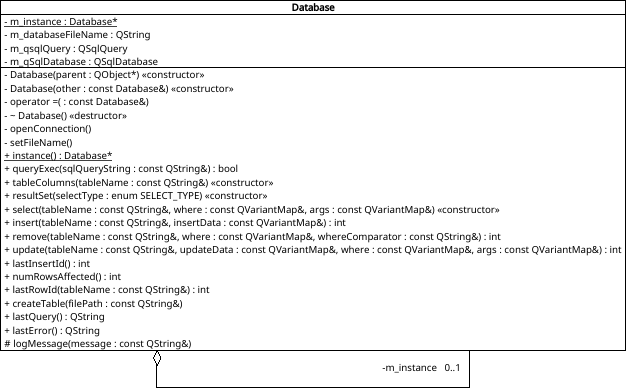
\includegraphics[width=8cm]{diagrama_de_classe_Database}
	\centering
	\caption{Diagrama da classe Database}
\end{figure}

\subsubsection{A classe DatabaseComponent}\label{sec:solucao-desenvolvida}
A classe \textit{DatabaseComponent} foi criada com o objetivo de fornecer um componente de alto nível que simplificasse para os plugins as operações em uma tabela específica. Essa classe será registrada no contexto da aplicação como um tipo QML com o nome de "\textit{Database}" e permitirá aos plugins utilizarem como componentes QML. \textit{DatabaseComponent} agrega uma instância da classe \textit{Database} e delega as operações para esse objeto. No entanto, ela possui alguns atributos declarados como \textit{Q\_PROPERTY} que permitem aos plugins informar o nome da tabela no banco de dados, uma coluna chave-primária do tipo string (quando a chave-primária não for numérica auto-incrementada), além de colunas que guardam objetos json. As colunas json evitam a realização de \textit{parsing} nas views ou \textit{delegates} para objetos agregados, sendo retornados já convertidos em objetos ou arrays.\par

Outro atributo \textit{totalItens} manterá atualizado o número de registros na tabela para fins de comparação com o número de itens disponível no serviço \textit{REST}, útil para paginação de dados na \textit{view}. O diagrama a seguir, apresenta os atributos e métodos dessa classe:

\begin{figure}[H]
	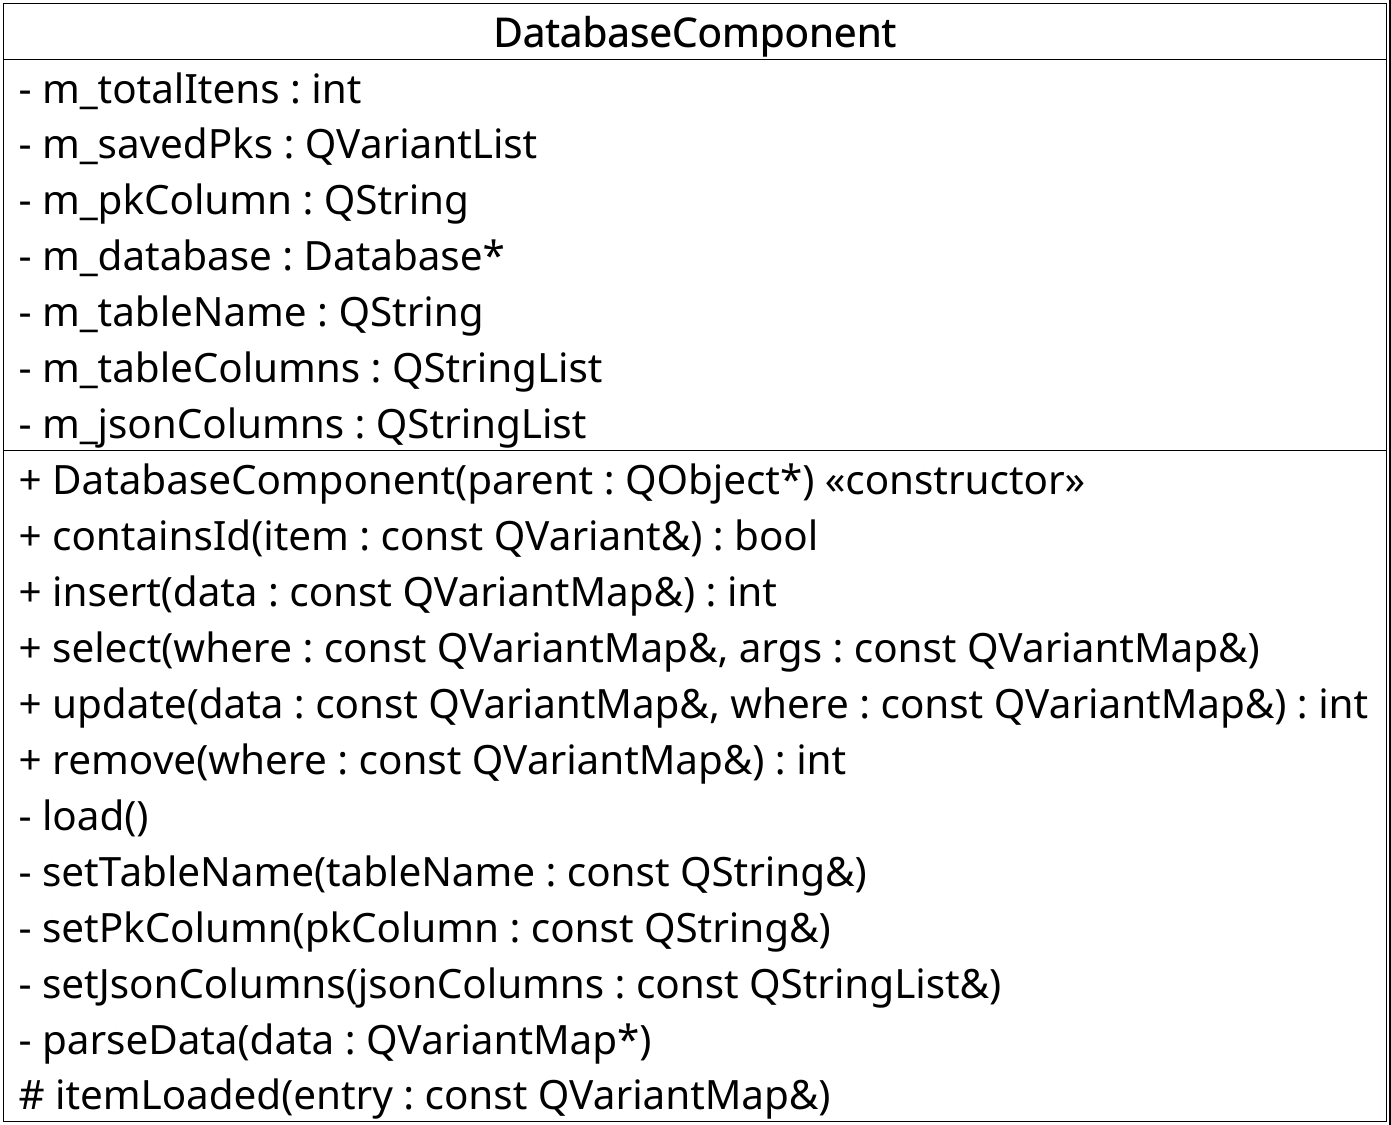
\includegraphics[width=8cm]{diagrama_de_classe_DatabaseComponent}
	\centering
	\caption{Diagrama da classe DatabaseComponent}
\end{figure}

É importante destacar que os métodos de busca, inserção, remoção e atualização foram simplificados para que os objetos informem apenas os parâmetros do método sem o nome da tabela. Outro recurso importante desse componente é que o método de busca é assíncrono e os resultados de uma busca, quando houver, serão retornados através do sinal \textit{itemLoaded} que passará como argumento um objeto no estilo \textit{nome-da-coluna.valor}. \textit{DatabaseComponent} possui ainda o método \textit{containsId} que verifica se um item (pela chave primária) já está salvo localmente e pode ser útil para sincronizar com a \textit{view} os itens já baixados do serviço \textit{REST}. O código a seguir, apresenta um exemplo de como um plugin poderá utilizar \textit{DatabaseComponent} para persistir dados em uma tabela:

\begin{center}
\begin{lstlisting}[language=qml]

import Database 1.0
...
Database {
	id: database
	jsonColumns: ["source"]
	tableName: "news"
	pkColumn: "title"
	onItemLoaded: listViewModel.append(entry)
}
...
Item {
	Component.onCompleted: {
		var args = {
			title: "GNU is not Unix!",
			message: "GNU is an operating...",
			datetime: "2017-12-30T14:29:33"
			source: {
				url:"https://foo.com/api",
				code:"foo",
				value:"bar"
			}
		}
		database.insert(args)
	}
}
...
\end{lstlisting}
\captionof{lstlisting}{Exemplo de como utilizar \textit{DatabaseComponent}}
\end{center}


\subsection{Notificações do Aplicativo}
O terceiro requisito funcional disponibilizado nesta arquitetura é o envio de notificação ao usuário do aplicativo e consiste de notificações via \textit{push} e local. As notificações via \textit{push} é suportado apenas no Android e iOS e as notificações locais é suportado nos dispositivos móveis além de linux desktop e MacOS. As notificações podem ser utilizadas para alertar o usuário de algum evento na aplicação e pode conter um título, uma descrição e nas plataformas mobile, pode vibrar o dispositivo e emitir um som. Outro recurso disponibilizado nas notificações é a possibilidade de adicionar algum dado extra em cada notificação. Esse dado deve ser um objeto \textit{chave.valor} e o valor pode ser tanto uma string como um valor numérico ou, outro objeto ou array. As notificações locais serão enviadas pela própria aplicação via chamada de método e as notificações via \textit{push} através do \textit{Firebase}. As subseções a seguir, descrevem detalhes de cada tipo de notificação.

\subsubsection{Notificações via push}
O suporte a notificações via \textit{push} já está configurado na arquitetura e o que o desenvolvedor deve fazer para enviar mensagens via \textit{push} é criar um projeto no \textit{Firebase}, exportar o arquivo \textit{google-services.json} e adicioná-lo no diretório \textit{android} e o arquivo \textit{google-services.xml} correspondente ao iOS no diretório \textit{ios}, substituindo os arquivos existentes, ambos criados como exemplo. É importante destacar que o \textit{package name} do aplicativo adicionado no \textit{AndroidManifest.xml} e o \textit{CFBundleIdentifier} no \textit{Info.plist} do iOS, devem ser o mesmo utilizado ao criar o projeto no \textit{Firebase}. Caso contrário, ocorrerá um erro ao construir o APK ou IPA, pois as bibliotecas correspondentes ao serviço de \textit{push} (adicionadas ao projeto durante o \textit{build}) farão um \textit{parsing} dos arquivos e abortará a compilação caso ocorra algum erro. No android, o \textit{package name} deve ser adicionado manualmente no arquivo \textit{build.gradle} presente no diretório \textit{android} na propriedade \textit{defaultConfig.applicationId}.\par

No android, o funcionamento de \textit{push notification} requer duas classes java que serão instanciadas na inicialização do aplicativo e funcionarão como dois serviços. Essas classes já estão na arquitetura e o desenvolvedor não precisa modificá-las. O primeiro serviço registra o dispositivo no \textit{Firebase} e retorna um token. Quando isso ocorrer, o token será passado para a aplicação através do sinal \textit{eventNotify} do objeto \textit{App}. O segundo serviço é um \textit{listener} de notificações via \textit{push} e ficará em execução mesmo que a aplicação seja fechada. Ao enviar uma notificação utilizando o console do \textit{Firebase} ou através de algum \textit{web service}, as notificações serão recebidas nesse serviço e enviadas para o \textit{system tray} automaticamente. Se o aplicativo estiver em execução, a notificação será encaminhada para o aplicativo em um objeto json contendo todos os dados da mensagem: o título, a data e a hora de envio e o dado de \textit{payload} (um dado adicional não visível enviado na mensagem).\par

No iOS, o arquivo \textit{QtAppDelegate.mm} presente no diretório \textit{ios} realizará o registro do dispositivo no \textit{Firebase} e contém um método que receberá as notificações via \textit{push} e re-encaminhará para a aplicação usando o mesmo sinal utilizado no android. Em ambas as plataformas, o token será passado para a aplicação através do evento \textit{newPushNotificationToken} e as mensagens de push, no evento \textit{newPushNotification}. Se a aplicação estiver em execução e o usuário clicar em uma notificação colocando o aplicativo em foreground, o evento \textit{newActionNotification} será disparado passando como argumento do evento os dados de \textit{payload} da mensagem.\par

A arquitetura dispõe do plugin de exemplo \textit{Listeners} que contém o componente \textit{PushNotificationRegister.qml}. Esse componente demostra um exemplo de como obter o token de registro no \textit{Firebase} e enviar para o serviço \textit{REST}, destruindo o componente (para otimizar consumo de memória) quando o token for recebido com sucesso pelo servidor.

\begin{center}
\begin{lstlisting}[language=qml]
import QtQuick 2.8

Connections {
    target: App
    onEventNotify: {
		var e
		e = Config.events.newPushNotificationToken
		if (e == eventName) {
			// enviando o token para o web service
			// eventData eh o argumento do evento
			// contendo uma string com o token
			sendTokenToServer(eventData)
		}
	}
}
\end{lstlisting}
\captionof{lstlisting}{Exemplo de como acessar o token do \textit{Firebase}}
\end{center}

\subsubsection{Notificações local}
Para gerenciar as notificações locais, foi criado a classe \textit{Notification} que abstrai a plataforma e dispõe de um método para enviar uma notificação para a área de notificações do sistema em execução. Essa classe será instanciada na inicialização do aplicativo e registrada no contexto da aplicação para que os plugins possam invocar o método \textit{Notification.show}, passando o título e a mensagem da notificação e opcionalmente um objeto contendo o argumento a ser passado para a aplicação quando o usuário clicar na notificação. Quando o usuário clicar na notificação, o aplicativo ficará em \textit{foreground} (caso não esteja) e o argumento da notificação será passado para o objeto \textit{App} que notificará a aplicação via \textit{eventNotify} contendo em \textit{eventName} a string \textit{newActionNotification} e em \textit{eventData}, o argumento passado no método \textit{show}. O código a seguir, apresenta um exemplo de como exibir uma notificação local por algum objeto de um plugin, passando um título, uma mensagem e um objeto como argumento.

\begin{center}
\begin{lstlisting}[language=qml]
import QtQuick 2.8

Item {
    Component.onCompleted: {
		var title = "Novo item carregado!"
		var message = "Clique para visualizar!"
		var argument = {
			key:"foo",
			value:"bar"
		}
		Notification.show(title,message,argument)
	}
}
\end{lstlisting}
\captionof{lstlisting}{Exemplo de como exibir uma notificação local}
\end{center}


\subsection{Comunicação entre os objetos e plugins}
% Esta seção descreverá o processo de comunicação entre objetos no aplicativo e o uso correto dos eventos...
O quarto requisito funcional desta arquitetura é a disponibilização de um mecanismo de comunicação entre objetos e plugins facilitado. A seção 4.9 descreveu o uso do sinal \textit{eventNotify} do objeto \textit{App}, utilizado por componentes internos e pelos plugins disponibilizados como exemplo na arquitetura. Porém, esse não é o único mecanismo de comunicação disponibilizado, a arquitetura dispõe de uma implementação em C++ do padrão de projeto \textit{Observer} baseado em categorias de eventos. A categoria, neste caso, é uma string que identifica um evento específico e visa notificar apenas os objetos interessados, evitando o \textit{broadcast} na aplicação em que todos os observadores da serão notificados. A implementação do \textit{Observer} permite ainda enviar um argumento para o objeto observador.\par

A implementação do Observer foi feito por duas classes C++, uma chamada \textit{Subject} e outra \textit{Observer}. Na inicialização da aplicação, a classe \textit{Subject} será instanciada e o objeto registrado no contexto da aplicação. A classe \textit{Observer} será registrada na aplicação como um tipo QML para que os plugins possam utilizá-lo como componente. A classe \textit{Subject} possui um atributo privado \textit{attacheds}, uma instância da classe \textit{QMap} do Qt que guardará um vetor de observadores para cada string que identifica um determinado evento. Quando um objeto deseja observar um evento, ele deve informar o nome do evento e passar uma referência para o observer que será informado quando o evento for disparado. Quando um determinado objeto deseja notificar observadores, ele invocará o método \textit{Subject.notify} passando no primeiro parâmetro uma string que identifica o evento, seguido de um objeto como argumento a ser passado para os observadores e por último, uma referência para sí mesmo que identificá como emissor do evento.

O objeto \textit{Subject} (registrado no contexto da aplicação) disponibiliza os seguintes métodos:

\begin{itemize}
	\item \textit{attach} (void): Esse método poderá ser utilizado para adicionar observadores a uma lista de eventos na aplicação e dois parâmetros são requeridos: o primeiro é um ponteiro para o \textit{observer} e o segundo, é uma lista de strings contendo os eventos que o observador deseja ser notificado;

	\item \textit{detach} (void): Esse método poderá ser utilizado para remover um observado de uma lista de eventos na aplicação e dois parâmetros são requeridos: o primeiro é um ponteiro para o \textit{observer} e o segundo é a lista de eventos da qual o observador será removido;

	\item \textit{notify} (void): Esse método poderá ser utilizado por qualquer objeto da aplicação para notificar observadores de um determinado evento. Esse método requer três parâmetros, o primeiro é uma string contendo o nome do evento, o segundo é um objeto variante contendo o dado a ser passado para o observador e por último um ponteiro \textit{QObject} para o emissor do evento. Ao chamar esse método, o \textit{Subject} irá iterar o vetor de observadores correspondente ao evento enviado, chamando para cada observador o método público \textit{update} que receberá como argumento, o nome do evento em que está sendo notificado, o argumento enviado e uma referência para o objeto emissor.
\end{itemize}

Os eventos podem ser adicionados no arquivo de configuração na propriedades \textit{events} e utilizá-los na aplicação através do objeto \textit{Config}. Os eventos devem formar um par de strings no estilo \textit{nome-do-evento.valor}, por exemplo: \textit{Config.events.foo}. Outro detalhe é que \textit{Subject} criará uma \textit{thread} para cada \textit{observer} quando for notificá-los de algum evento. Isso significa que a chamada ao método \textit{update} em cada \textit{observer} será assíncrono para garantir o melhor desempenho. O código a seguir, apresenta um exemplo de como utilizar o \textit{Observer} por objetos nos plugins.

\begin{center}
\begin{lstlisting}[language=qml]
import Observer 1.0
...
Observer {
	id: observer
	events: [Config.events.newSourceAdded]
	onUpdated: database.insert(eventData)
}
...
Item {
	Component.onCompleted: {
		// pede ao Subject para adicionar
		// o observador a lista do evento
		var event = Config.events.newSourceAdded
		Subject.attach(observer, event)
	}
}
...
\end{lstlisting}
\captionof{lstlisting}{Exemplo de como utilizar o \textit{Observer}}
\end{center}

O código a seguir, apresenta um exemplo de como notificar observadores de um determinado evento:

\begin{center}
\begin{lstlisting}[language=qml]
import QtQuick 2.8
...
Item {
	id: rootItem
	Component.onCompleted: {
		var event = Config.events.newSourceAdded
		var args = {
			key:"foo",
			value:"bar"
		}
		Subject.notify(event, args, rootItem)
	}
}
\end{lstlisting}
\captionof{lstlisting}{Exemplo de como notificar observadores}
\end{center}


\subsection{O perfil de usuário}\label{sec:solucao-desenvolvida}
A arquitetura dispõe o componente \textit{UserProfile.qml} para gerenciar os dados do usuário do aplicativo, ele será instanciado na inicialização da aplicação e setado no objeto \textit{userProfile} se houver login na aplicação, ou seja, se o desenvolvedor definir nas configurações a propriedade \textit{usesLogin} para \textit{true}. Esse objeto (\textit{userProfile}) estará disponível para os plugins como um objeto global, e a propriedade \textit{profile} poderá ser utilizada em \textit{bindings} com outros objetos. No entando, atualizações no perfil do usuário não devem ser feitas diretamente no objeto profile e sim, através de eventos.\par

O componente \textit{UserProfile.qml} observará três eventos na aplicação pelo qual os plugins devem utilizá-los para setar ou editar as informações do usuário. O primeiro evento \textit{initUserProfile}, poderá ser utilizado para inicializar o perfil do usuário após o login e o argumento do evento deve conter um objeto enviado pelo serviço \textit{REST} contendo no mínimo os campos \textit{id} e \textit{email}. O segundo evento \textit{setUserProfileData}, deve ser utilizado para atualizar ou adicionar alguma informação ao perfil do usuário. Nesse evento, o argumento deve conter as propriedades \textit{key} com o nome do campo a ser atualizado (ou adicionado) e \textit{value} a informação para o campo correspondente. O terceiro evento \textit{logoutApplication}, deve ser disparado pela página de \textit{logout} para avisar que a seção foi encerrada e o usuário será direcionado para a página de login. No \textit{logout}, o argumento do evento pode ser \textit{false} ou simplesmente \textit{null}. O componente \textit{UserProfile} dispõe das seguintes propriedades:

\begin{itemize}
	\item \textit{profile} (object): Um objeto javascript que guardará os dados do perfil do usuário, no estilo \textit{campo.valor}. Os plugins podem fazer \textit{binding} com esse objeto em elementos visuais tais como, exibir a imagem de perfil através do campo \textit{image\_url} (via \textit{profile.image\_url}). Esse objeto será persistido a cada alteração;

	\item \textit{profileName} (string): Uma string contendo o nome do perfil do usuário, por exemplo, \textit{administrator}, \textit{editor}, \textit{student} e etc. Essa propriedade será setada internamente quando o \textit{profile} for definido ou alterado. No entanto, o nome do perfil do usuário deve ser passado pelo serviço \textit{REST} na resposta do login. É importante destacar que essa propriedade será definida somente se o serviço \textit{REST} adicionar no objeto (do perfil do usuário, retornado no login) a propriedade \textit{user\_role.name}, que é o valor atribuído a essa propriedade. A exibição das páginas para o usuário será baseado nessa propriedade através de \textit{bindings}. Se a propriedade \textit{roles} na configuração das páginas dos plugins for definido e \textit{profileName} for uma string vazia o usuário não visualizará as páginas no menu do aplicativo;

	\item \textit{isLoggedIn} (bool): Essa propriedade será definida para \textit{true} quando \textit{profile} for modificado contendo alguma informação válida, ou seja, \textit{id} e \textit{email} (no mínimo). \textit{isLoggedIn} será \textit{false} quando não houver informações em \textit{profile}. Essa propriedade será modificada internamente após os eventos \textit{initUserProfile} e \textit{logoutApplication}. \textit{isLoggedIn} será persistida sempre que for modificada.
\end{itemize}

O objeto \textit{userProfile} invocará uma função interna que carregará a página inicial (\textit{home page}) após \textit{profile} ser modificado, ou seja, após o evento \textit{initUserProfile}. A página de login também será carregada após o evento \textit{logoutApplication}. A arquitetura disponibiliza o plugin de exemplo \textit{Session} e alguns arquivos que demonstram a utilização do \textit{login}, \textit{logout}, exibição do perfil e como solicitar alterações nos dados do usuário através do evento \textit{setUserProfileData} (o arquivo ProfileEdit.qml).\par

É importante destacar, que após o sucesso do primeiro login, não será necessário logar novamente na próxima inicialização, pois, as informações do usuário serão persistidas e na próxima inicialização o carregamento da primeira página será feita de acordo com o valor definido \textit{isLoggedIn}. Se o login for efetuado com sucesso na execução anterior, essa propriedade será \textit{true}, pois ela inicializará com o último valor definido na execução anterior.\par

O código a seguir, apresenta um exemplo de como utilizar o perfil do usuário através do objeto \textit{userProfile}.

\begin{center}
\begin{lstlisting}[language=qml]
import QtQuick 2.8
...
Column {
	spacing: 10

	// userProfile eh um objeto global,
	// criado e declarado no main window!
	property var profileData = userProfile.profile

	// exibindo a imagem de perfil
	Image {
		id: userImg
		asynchronous: true; cache: true
		source: profileData.image_url
	}

	// exibindo o email do usuario
	Label {
		id: userEmail
		text: profileData.email
	}
}
\end{lstlisting}
\captionof{lstlisting}{Exemplo de como exibir informações do usuário}
\end{center}


\subsection{O Componente BasePage.qml}\label{sec:solucao-desenvolvida}
O componente \textit{BasePage} é um arquivo genérico que fornece algumas propriedades para as páginas dos plugins, além de fazer \textit{bindings} com o \textit{ToolBar}, o \textit{TabBar}. \textit{BasePage} deverá ser utilizada pelas páginas de plugins sempre que possível. Esse componente irá instanciar um \textit{ListView} contendo um \textit{ListModel} e um \textit{RequestHttp} para facilitar o trabalho do programador e reduzir a escrita de código pelos plugins. \textit{BasePage} pode ser visto como uma classe abstrata que possui alguns atributos e métodos agregados. As propriedades a seguir, compõem o \textit{BasePage} e devem ser utilizadas para customizar a estrutura das páginas.

\begin{itemize}
	\item \textit{toolBarButtons} (array): uma lista de objetos contendo as propriedades de um botão \textit{ToolBarButton} a serem adicionados no \textit{ToolBar} dinamicamente quando a página for carregada. Cada objeto deve conter as seguintes propriedades: \textit{iconName}, uma string contendo o nome de um ícone do \textit{Awesome Icons} e \textit{callback} uma função javascript que será invocada quando o botão for pressionado pelo usuário;

	\item \textit{toolBarState} (string): essa propriedade poderá ser utilizada para definir o estado do \textit{ToolBar} e três valores estão disponíveis. O primeiro deles é \textit{normal} que é o valor \textit{default}. O segundo valor é \textit{goBack} e quando for utilizado, permitirá ao usuário sair da página atual e retornar para a página anterior clicando em uma seta para a esquerda, essa seta será adicionada pelo \textit{ToolBar}. O último valor é \textit{search} que exibirá um campo de busca no \textit{ToolBar} permitindo ao usuário digitar um texto para pesquisar algo na \textit{view} (página corrente). No modo \textit{seach}, a propriedade \textit{searchText} também de \textit{BasePage} receberá uma cópia do texto digitado pelo usuário;

	\item \textit{absPath} (string): essa propriedade deverá ser definida pela página para que o menu declare um \textit{bind} entre o item correspondente (na lista de itens do menu, tornado-o selecionado) com a página atualmente vista pelo usuário. Para setar essa propriedade, a página poderá utilizar o nome do plugin a partir do objeto \textit{Config.plugins} + o nome do arquivo QML correspondente. Por exemplo, considerando um plugin chamado \textit{LoadMessages} e a página \textit{View.qml}, essa propriedade pode ser definida da seguinte forma: \textit{absPath: Config.plugins.loadmessages + "View.qml"};

	\item \textit{showToolBar} (bool): essa propriedade deverá ser utilizada se a página deseja ocultar o menu do layout em pilha, que é uma instancia do \textit{ToolBar} do \textit{QuickControls};

	\item \textit{showTabBar} (bool): essa propriedade deverá ser utilizada quando a página precisar ocultar o menu do layout em linha, que é uma instancia do \textit{TabBar} do \textit{QuickControls};

	\item \textit{hasNetworkRequest} (bool): essa propriedade é \textit{true} por \textit{default} e se mantida com o valor padrão, instanciará um objeto \textit{RequestHttp.qml} quando a página for carregada. Outra propriedade de \textit{BasePage} \textit{requestHttp} receberá uma referência para esse objeto e poderá ser utilizada pela página para fazer requisições HTTP. No entanto, se a página não realizará requisições HTTP, deverá setar \textit{false} para essa propriedade;

	\item \textit{hasListView} (bool): essa propriedade é \textit{true} por \textit{default} e se mantida com o valor padrão, instanciará um \textit{ListView} do \textit{QuickControls} e passará a referência para a propriedade \textit{listView}. O \textit{ListView} já terá um \textit{ListModel} do QML que será atribuído a propriedade \textit{listViewModel} também de \textit{BasePage} e poderá ser utilizada pela página para fazer \textit{append} ou remover itens da \textit{view};

	\item \textit{isPageBusy} (bool): essa propriedade é \textit{false} por \textit{default} e fará um \textit{bind} com o status de cada requisição HTTP feita pela página quando o objeto \textit{RequestHttp} for instanciado. Logo, o \textit{bind} será criado somente se a página manter \textit{hasNetworkRequest} como \textit{true};

	\item \textit{isActivePage} (bool): essa propriedade fará um \textit{bind} com o \textit{window.currentPage} que é uma referência para a página atualmente vista pelo usuário;

	\item \textit{listViewDelegate} (Component): essa propriedade é \textit{null} por \textit{default} e deve ser definida pela página quando utilizar \textit{ListView} atribuindo ao \textit{delegate} correspondente. Quando o \textit{ListView} for instanciado, essa propriedade será atribuída a \textit{delegate} do \textit{ListView};

	\item \textit{pageBackgroundColor} (Color): essa propriedade pode ser utilizada para definir uma cor de fundo personalizada para a página, pode ser tanto hexadecimal como RGBA. A cor padrão utilizada será o valor definido no arquivo de configuração na propriedade \textit{theme.pageBackgroundColor}.
\end{itemize}

É importante destacar que \textit{BasePage} \textit{extends} o componente \textit{Page} do \textit{QuickControls} e as propriedades definidas em \textit{Page} serão herdadas, como por exemplo, \textit{title}, que deve ser definido pela página para exibir ao usuário o título da página que ele está visualizando. Para utilizar \textit{BasePage}, basta adicionar a diretiva \textit{import "qrc:/publicComponents"} e declarar um objeto \textit{BasePage} como no exemplo a seguir:

\begin{center}
\begin{lstlisting}[language=qml]
import QtQuick.Controls 2.0
import "qrc:/publicComponents/" as Components

Components.BasePage {
	id: page

	// ignora o uso do ListView
	hasListView: false

	// define o path absoluto
	absPath: Config.plugins.pages + "Page1.qml"

	// exibe um titulo no ToolBar
	title: qsTr("Page 1")

	// permite sair da pagina atual
	// usando o botao voltar no ToolBar
	toolBarState: "goBack"

	// trata as respostas de um pedido http
	onRequestFinished: {
		console.log("status:", statusCode)
		console.log("response:" , response)
	}
...
}
\end{lstlisting}
\captionof{lstlisting}{Exemplo de uso do \textit{BasePage}}
\end{center}


\subsection{Componentes Reusáveis}\label{sec:solucao-desenvolvida}
A arquitetura dispõe de quinze componentes reusáveis para os plugins, há componentes visuais e não visuais e para utilizá-los basta adicionar a diretiva \textit{import "qrc:/publicComponentes/"} e declarar como componente QML. Os componentes disponíveis serão descritos a seguir:

\begin{itemize}
	\item \textit{ActionMessage.qml}: esse componente exibe um botão contendo um texto e um ícone do \textit{Awesome Icons} no centro da tela. O texto pode ser definido na propriedade \textit{messageText} e o ícone na propriedade \textit{iconName}. O ícone e o texto estão disposts em um \textit{ColumnLayout} sendo o ícone acima do texto. Dois sinais serão emitidos: \textit{clicked()} e \textit{pressAndHold()} quando clicado e pressionado respectivamente pelo usuário;

	\item \textit{AwesomeIcon.qml}: esse componente consiste de um \textit{RoundButton} do \textit{QuickControls} com a propriedade \textit{flat} setado para \textit{true} para que o background seja transparente. Ele utiliza um arquivo de fonte OTF contendo setessentos e vinte ícones da biblioteca \textit{Awesome Icons} e poderá ser utilizado para exibir um ícone clicável nos fragmentos de uma página. As propriedades \textit{name}, \textit{size} e \textit{color} podem ser utilizadas para definir o ícone, o tamanho e a cor;

	\item \textit{BasePage.qml}: esse componente é o elemento descrito na seção anterior e deve ser utilizado pelos plugins nas páginas no aplicativo;

	\item \textit{Brand.qml}: esse componente consiste de um retângulo e uma imagem centralizada. A imagem utilizada é por padrão o ícone definido em \textit{assets/icon.png}. O plugin \textit{About} fornecido como exemplo, utiliza esse componente no topo da tela para exibir a logo do aplicativo;

	\item \textit{CameraCapture.qml}: esse componente pode ser utilizado para abrir a câmera do dispositivo móvel ou a \textit{webcam} em laptops. Ao adicionar esse componente no \textit{StackVIew}, ele inicializará a câmera disponível no dispositivo e permitirá ao usuário capturar uma imagem clicando em qualquer ponto da tela ou, utilizando o botão \textit{photo} no rodapé da janela. Outros dois botões estarão disponíveis nos cantos da tela. O botão do lado esquerdo permitirá ao usuário alternar entre as câmeras frontal ou de fundo (se disponível), e o do lado direito, abre a janela para seleção de arquivos no dispositivo. Se o usuário capturar uma imagem com a câmera, a imagem capturada será salva em um diretório público do dispositivo e o evento \textit{cameraImageSaved} será disparado contendo como argumento do evento, uma string com o \textit{path} da imagem;

	\item \textit{CustomButton.qml}: esse componente consiste de um botão com as bordas arredondadas e com a paleta de cores definida para: \textit{colorPrimary} como cor de fundo, \textit{colorControlHighlight} como cor da borda e \textit{colorAccent} como cor do texto. Essas cores devem ser definidas pelo programador no arquivo de configuração na propriedade \textit{theme};

	\item \textit{CustomListView.qml}: esse componente \textit{extends} o \textit{ListView} do \textit{QuickControls} e já dispõe de um \textit{ListModel} que será instanciado e definido como model do \textit{ListView}. Também será adicionado efeitos de transição (quando um item for adicionado ou removido), além de um objeto \textit{ScrollIndicator} que exibirá uma barra de rolagem vertical dinamicamente;

	\item \textit{Datepicker.qml}: esse componente pode ser utilizado para exibir um caledário contendo opção de seleção de dia, mês e ano. Após o usuário selecionar uma data, o sinal \textit{dateSelected(int day, int month, int year)} será emitido pelo objeto;

	\item \textit{FloatingButton.qml}: esse componente exibe um botão circular flutuante no lado direito da tela, no rodapé da janela do aplicativo. É possível definir um ícone do \textit{Awesome} através da propriedade \textit{iconName} e possui os mesmos sinais de um \textit{Button} do \textit{QuickControls}, tais como o \textit{clicked} e \textit{pressAndHold};

	\item \textit{ListItem.qml}: esse componente é um \textit{ItemDelegate} do \textit{QuickControls} e permite adicionar até quatro elementos visuais, além de uma borda no rodapé que será utilizada como separador em uma lista de elementos. A utilização desse componente pode ser feita tanto como \textit{delegate} de um \textit{ListView} como em uma página dentro de um \textit{ColumnLayout}.\par
	Os elementos visuais são: um ícone do \textit{Awesome Icon} através da propriedade \textit{primaryIconName} ou uma imagem setando o \textit{source} na propriedade \textit{primaryImageSource} e será posicionado no lado esquerdo e centralizado verticalmente.\par
	Ao lado direito do ícone (lateral esquerdo, se for definido), pode ser adicionado um texto e uma descrição através das propriedades \textit{primaryLabelText} e \textit{secondaryLabelText} respectivamente, um abaixo do outro, sendo a descrição com o \textit{font-size} e opacidade reduzidos. O último elemento visual, é o mesmo do primeiro só que, posicionado no lado direito e pode ser um ícone do \textit{Awesome Icon} ou uma imagem. A imagem em ambos os lados pode ser um endereço remoto ou a partir do \textit{qrc};

	\item \textit{PasswordField.qml}: esse componente \textit{extends} o \textit{TextField} do \textit{QuickControls} e pode ser utilizado para exibir um campo de senha para o usuário, contendo um ícone do \textit{Awesome} ao lado direito centralizado verticamente. O ícone permitirá exibir a senha digitada no campo quando for clicado, alternando o valor da propriedade \textit{echoMode} entre \textit{Password} ou \textit{Normal};

	\item \textit{PhotoSelection.qml}: esse componente é um \textit{Popup} do \textit{QuickControls} e pode ser utilizado para exibir uma lista vertical de opções clicáveis para o usuário, três opções estão disponíveis: A primeira opção, ao ser clicada, abre a câmera do dispositivo, ou seja, irá instanciar \textit{CameraCapture.qml}. A segunda opção abrirá a galeria de imagens do dispositivo para seleção de um único arquivo. A terceira opção, ao ser clicada, nada será feito internamente, apenas emitirá o sinal \textit{removeCurrentPhoto} para que algum plugin possa executar essa ação de remover a imagem de perfil do usuário;

	\item \textit{RequestHttp.qml}: esse componente já foi apresentado na seção que descreve a API de rede e deve ser utilizado quando for necessário realizar requisições HTTP. É importante lembrar que \textit{BasePage} já possui uma instância desse componente permitindo as páginas iniciar requisições ao serviço \textit{REST}. No entanto, esse componente pode ser utilizado em objetos \textit{listeners};

	\item \textit{RoundedImage.qml}: esse componente exibe uma imagem arredondada e dispõe as propriedades \textit{imgSource} para o \textit{path} da imagem (local ou remota) e \textit{borderColor} para definir uma cor para a borda (o padrão é transparente). A imagem será adicionada em um retângulo com um \textit{MouseArea}, tornando possível capturar eventos de \textit{click} ou pressionamento na imagem;

	\item \textit{TimePicker.qml}: esse componente exibirá um relógio baseado em \textit{hora:minuto:segundos}. Ele \textit{extends} \textit{Popup} do \textit{QuickControls} e para abrir o diálogo, é preciso chamar o método \textit{open()} a partir do objeto declarado. Quando o usuário selecionar a hora e clicar no botão \textit{OK}, o sinal \textit{timeSelected(var time)} será emitido.
\end{itemize}


\subsection{Fluxo de execução}\label{sec:solucao-desenvolvida}
A figura exibida no final desta seção, demonstra o \textit{workflow} de um aplicativo baseado nesta arquitetura. As aplicações Qt possuem nas plataformas mobile, objetos \textit{Java} e \textit{ObjectiveC} no android e iOS respectivamente, que inicializam o aplicativo em cada plataforma e em seguida executam a aplicação tendo como ponto de entrada o \textit{main.cpp}.\par

Os elementos visuais serão carregados no \textit{main.qml} que será instanciado no último passo antes de iniciar o \textit{loop} da aplicação. O \textit{main.qml} corresponde a \textit{ApplicationWindow} do \textit{QuickControls} e poderá ser acessado por qualquer objeto através do id \textit{window}. Os \textit{listeners} serão carregados quando \textit{window} estiver pronto e poderão acessar qualquer uma das propriedades declaradas no escopo do \textit{window}, tais como \textit{userProfile}. O \textit{window} contém dois \textit{widgets} que podem ser utilizados para exibir avisos ao usuário. Os \textit{widgets} são \textit{Snackbar} e \textit{Toast} e foram inspirados nos respectivos componentes do \textit{Material Design}. Os \textit{widgets} dispõe da função \textit{show} que exige uma string como parâmetro, essa string será o texto exibido ao usuário.\par

A figura a seguir, apresenta de uma forma resumida o fluxo de inicialização e a sequência de objetos instanciados em um aplicativo baseado nesta arquitetura.

\begin{figure}[H]
	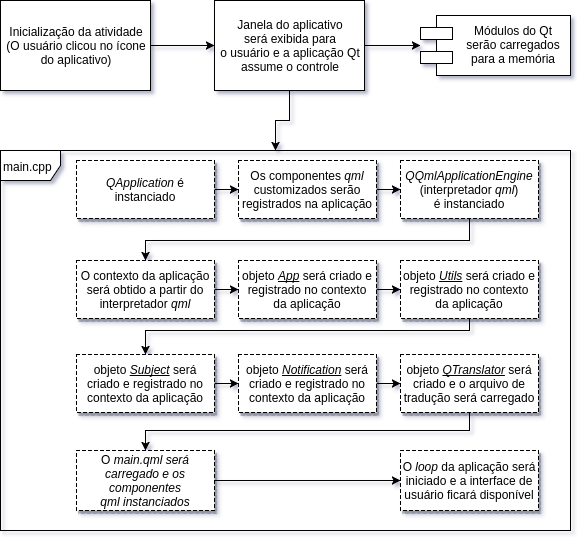
\includegraphics[width=8cm]{diagrama_fluxo_execucao}
	\centering
	\caption{\textit{workflow} da execução de um aplicativo Qt}
\end{figure}


\subsection{Métodos para utilização da arquitetura}
% descrever o README do projeto no github
Para se utilizar a arquitetura desenvolvida, deve-se seguir uma determinada ordem de atividades que serão descritos a seguir...